%=========================================================================
% (c) Michal Bidlo, Bohuslav Křena, 2008
%\setcounter{secnumdepth}{4} % cislovani nadpisu do hloubky



\chapter{Úvod}
\label{chapter:1}

V současné době se technologie ve všech odvětvích stále posouvá a~není tomu jinak ani u~prohlížení fotografií a~videí. I~takto nahrané informace pomocí digitálních zařízení je trend dále posouvat a~zvyšovat tak zážitek ze zaznamenané události. Díky tomuto trendu si už nevystačíme s \uv{klasickými} přehrávači, popř. prohlížeči videí nebo fotografií. Díky sférickým 360 stupňovým kamerám je dnes možné zaznamenat video o~srovnatelné velikosti jako u dnes běžného telefonu, ale s~mnohem větším objemem informací, které se však nedají srozumitelně přehrát v~klasických přehrávačích. Ruku v ruce se sdílením takových dat je velice výhodné takový prohlížeč nabídnout jako webovou verzi, aby i~jiní uživatelé mohli svá takto natočená videa přehrávat, popř. sdílet. Důkazem toho je rozmach multimediálního obsahu na internetu, kdy samotný jazyk HTML pro prezentaci webových stránek dříve nenabízel přímou podporu videí, což se změnilo příchodem nové verze HTML5. Některé portály jako např. Youtube již dnes začíná nasazovat do svého prohlížení videí jeho rozšířené sférické verze, což tedy potvrzuje tento trend. Tato práce má za cíl takové prohlížení posunout ještě dál.


Následující práce se věnuje implementaci webového prohlížeče panoramatických snímků a videí v různých módech, ve kterých je video interpretováno. Cílem je  navrhnout a zrealizovat řešení, aby uživatel po natočení videa dále nepotřeboval k přehrání specifický program. Zvláště v případě  sférického videa v režimu rybího oka, kdy uživatel nejprve musí video překonvertovat do ekvidistantního zobrazení, aby jej mohl sféricky prohlížet. Díky řešení v následujících kapitolách tato nutnost odpadá. 


Další inovací v prohlížení videí je přidání některých dat, které v běžném prohlížení nejsou k dispozici. Například informace o světových stranách ve vztahu k obrázku či videu, popřípadě údaje o velikosti zorného pole v daném kontextu prohlížení až po dodatečná metadata v~panoramatických obrázcích, které jsou vhodné například k~tomu, aby autor obrázku mohl popsat jeho zajímavé části nebo blíže popsat zachycenou scénu a její okolnosti.
\newline

Samotná práce je členěna do šesti částí. V kapitole \nameref{chapter:2} se budu věnovat nastínění všech použitých technologií nutných pro pochopení problematiky, se kterými se bude pracovat v následujících kapitolách. O návrhu řešení pojednává kapitola \nameref{chapter:3}, na kterou navazuje implementační část \nameref{chapter:4}. Otestování správného návrhu a implementace se zabývá kapitola  \nameref{chapter:5}. V poslední části práce \nameref{chapter:6} jsou prezentovány dosažené výsledky a možnosti dalšího rozšíření.


%=========================================================================


\chapter{Webové technologie prohlížeče}
\label{chapter:2}
Následující kapitola pojednává o technologiích, které samotný prohlížeč používá a jsou tedy nezbytné v dalších kapitolách, zejména v části \nameref{chapter:4}, kde se s nimi přímo pracuje.


\section{HTML5}

Jazyk HTML (HyperText Markup Language) je značkovací jazyk určený pro popis webových stránek. Vychází z univerzálního značkovacího jazyka SGML (Standard Generalized Markup Language). V současné době aktuální verzí  jazyka HTML je jeho již pátá verze -  HTML5. Nová verze HTML přináší zásadní vylepšení, nové funkce a možnosti, které jsou nezbytné pro návrh a implementaci webového prohlížeče. 

Pro návrh samotného programu je nezbytná podpora multimédií – tedy audio a video, v neposlední řadě také plátno \texttt{<canvas>} sloužící pro práci s grafikou.



\subsection{Video}
Dříve nebylo možné do webových stránek vložit video tak jako dnes. K tomuto účelu bylo využíváno různých zásuvných modulů třetích stran a do webových stránek se video vkládalo např. jako objekt. Nejvíce rozšířeným přehrávačem videí a tedy jakási náhrada za podporu videí, kterou tehdy HTML nemělo, se v širším spektru stal Adobe Flash, který funkci přehrávače plní v menší míře až doposud, avšak je již zastíněn efektivnějším řešením, a to právě HTML5. \cite{HTML5aCSS3}

Nový prvek v HTML5 vytvořený k tomuto účelu je \texttt{<video>}. Byl navržen tak, aby mohl být použit bez detekčních skriptů na stránce. V elementu videa je možné nastavit více souborů s videem a dle podpory si daný prohlížeč vybere jim podporované video. V případě, že by prohlížeč prvek videa nepodporoval, bude jej ignorovat. Nastavení více zdrojů videa s odlišnými kodeky lze pomocí elementu \texttt{<source>} uvnitř páru elementů \texttt{<video>...</video>}. Jakmile prohlížeč narazí na \texttt{<video>}, podívá se, zdali je přítomen atribut \texttt{src}. V opačném případě začne procházet jeden element \texttt{<source>} po druhém a bude hledat právě takový, který umí přehrát.

Aby bylo možné ovládat video dynamicky pomocí kláves nebo myší, bude nutné využít DOM (Document Object Model). Jedná se o stromovou strukturu dokumentu, kterou si prohlížeč sestavuje po načtení webové stránky. Všechny elementy webové stránky jsou interpretovány v DOM jako objekt. Některé značky se v DOM vytvoří, aniž by byly ve zdrojovém kódu zapsány. Obecně platí, že prostřednictvím objektového modelu je díky javascriptu možné tuto stromovou strukturu dále upravovat a rozšiřovat. 



\subsection{Stavy načítání a přehrávání videa}
Další velice důležitou částí je načítáni videa a jeho ověření, zda je již video připraveno k přehrání. K ověření dostupnosti videa lze použít jeden ze síťových stavů elementu pomocí stavového atributu \texttt{networkState}, popřípadě přímo zjišťovat připravenost videa pomocí atributu \texttt{readyState} \cite{html5}, vracející jeden z následujících stavů, podle kterých se můžeme dále při přehrávání řídit a přizpůsobit tomu běh programu. Jednotlivé konstanty nabývají hodnot od \texttt{0} do \texttt{4} a dle hodnot rozlišujeme:


\begin{itemize}
	\item \texttt{HAVE\_NOTHING } (ekvivalentní hodnotě 0) \newline
	 - nastane v situaci, kdy zdrojové video není dostupné, nebo nejsou dostupná žádná data pro aktuální přehrávanou pozici \newline - koresponduje také s návratovou hodnotou síťové metody \texttt{networkState()} v případě, když její návratová hodnota je rovna \texttt{0}, což odpovídá konstantě \texttt{NETWORK\_EMPTY}.
	
	\item \texttt{HAVE\_METADATA} \newline
		-  základní data o videu se podařilo získat a zdroj je tedy považován jako dostupný. V tomto stavu ale ještě není dostatek dat, aby bylo možné začít s přehráváním. V aktuálním stavu jsou k dispozici jen data popisující přehrávaný subjekt. Jsou načteny údaje videa o jeho délce, šířce, dekódovaní apod. Dochází  také k vyvolání události \texttt{loadedmetadata}.\cite{html5}
	
	\item \texttt{HAVE\_CURRENT\_DATA }\newline
		- data jsou pro bezprostřední začátek přehrávání již  připravena, ale video ještě není načteno dál za tuto pozici. Přehrávání se může  dostat do stavu \texttt{HAVE\_METADATA}, nebo se také může stát, že  následující data videa již nejsou k dispozici.
	
	\item \texttt{HAVE\_FUTURE\_DATA}\newline
		- data pro přehrávání jsou připravena pro současnou i nadcházející pozici. V případě, že by video dosáhlo takového stavu poprvé, bude vyvolána událost \texttt{canplay}.
		
	\item \texttt{HAVE\_ENOUGH\_DATA}\newline
		- data jsou připravena pro aktuální i nadcházející pozice pro plynulé přehrání. Dochází k vyvolání události \texttt{canplaythrough}.
\end{itemize}

Mimo stavy načtení videa jsou tu i události indikující, co přesně se právě děje s videem po jeho načtení. Tyto stavy se hodí k dotazování elementu \texttt{<video>} pomocí DOMu pro tvorbu vlastního specifického ovládání videa nebo pro zahrnutí interakce s myší.



\begin{itemize}
	\item \texttt{playing} - video se aktuálně přehrává. Atribut \texttt{paused} je nastaven na \texttt{false}.	
	
	\item \texttt{waiting} - přehrávání videa je pozastaveno, protože následující data videa nejsou k dispozici, webový prohlížeč ale očekává, že je v vzápětí dostane.
	
	\item \texttt{ended} - přehrávání videa doběhlo nakonec
	
	\item \texttt{canplaythrough} - tato událost říká, že je možné video přehrát až do konce bez nutnosti video zastavit k dalšímu načítání. Tohoto stavu může dosáhnout jen v případě, že stavový atribut \texttt{readyState} je roven \texttt{HAVE\_ENOUGH\_DATA}.
	
\end{itemize}

%=========================================================================
\newpage

\subsection{Atributy videa}
Důležité atributy pro manipulaci s videem a nastavením.



\begin{description}
	\item[src] - jedná se o atribut, do kterého se definuje zdrojové adresa videa jako URL, které se má zobrazit. Používá se zejména v situaci, kdy je k dispozici právě jedna verze videa.
	
	\item[autoplay] - jedná se atribut typu \texttt{bool}. V případě, že je \texttt{true}, spustí se přehrávání média automaticky jakmile je vše připraveno. Uvedení názvu atributu do elementu samotného je již dostačující informace o tom, co se bude dít s videem. Tedy bude tato hodnota typu \texttt{bool} považována jako \texttt{true}, jinak \texttt{false}.	
	
	\item[poster]  - Slouží k vystihnutí obsahu daného videa ještě než začne samotné přehrávání. Je možné jako první snímek videa zvolit obrázek zadaný cestou. V~případe, že tento atribut nebude vyplněn, tak HTML automaticky zvolí jeden z prvních neprázdných rámců.
	
	\item[loop]  - jedná se atribut typu \texttt{bool}, který začne po dosažení konce videa s přehráváním videa opět od začátku. Tato operace se provádí v nekonečné smyčce.

	\item[width] - šířka přehrávače v pixelech.
	
	\item[height] - výška přehrávače v pixelech.

	\item[paused] - atribut videa typu \texttt{bool}. Indikuje, zdali se video přehrává či nikoliv.

	\item[controls] - jedná se opět o atribut typu \texttt{bool}, který říká, aby prohlížeč použil vlastní ovládací prvky pro video. Ovládací prvky se dají také vytvořit a přizpůsobit velice snadno díky DOMu.
 	
 	\item[preload]  - tímto říkáme, jakou část videa by měl webový prohlížeč načíst ihned po načtení stránky. Tento atribut nabývá jednou ze tří hodnot:
	 	\begin{itemize}
	 		\item \texttt{none} - nebude načítat nic. Výhodné v případě, kdy je potřeba minimalizovat vytížení pásma.	 		
	 		\item \texttt{metadata} - načte pouze metadata daného videa - základní údaje o jeho délce apod.
	 		\item \texttt{auto} - sám zvolí, co přesně udělá.
	 	\end{itemize}
\end{description}

%=========================================================================
\newpage

\subsection{Metody videa}
Jelikož pomocí DOM je možné upravovat vlastnosti elementu \texttt{<video>}, tak jsou tedy nutné metody k ovlivnění jeho atributů, aby bylo možné s přehráváním videa manipulovat.

\begin{description}
	\item[\texttt{play()}] - metoda sloužící k nastavení atributu \texttt{paused} na \texttt{false}. Pokud video již skončilo, začne je přehrávat od začátku.
	
	\item[\texttt{pause()}] - metoda sloužící k nastavení atributu \texttt{paused} na \texttt{true}, čímž dojde k pozastavení videa.
	
	\item[\texttt{canplaytype()}] - metoda sloužící k ověření, zdali webový prohlížeč dokáže video daného typu přehrát. Metoda vrací jednu z následujících hodnot:
	 	\begin{itemize}		
			\item \texttt{""} - pokud by metoda vrátila prázdný řetězec, video prohlížeč nedokáže přehrát.
			\item \texttt{maybe} - prohlížeč si není zcela jist, zdali dokáže formát přehrát.
			\item \texttt{probably} - daný formát videa dokáže prohlížeč přehrát s vysokou pravděpodobností.
		\end{itemize}
	\item[\texttt{load()}] - všechny data videa se načtou znovu, čímž dojde ke zrušení všech akcí a současných dat, které byly doposud staženy a načteny. Poté se vše zavolá a načte znovu následujícím způsobem:
	 	\begin{enumerate}
			\item Nejprve dojde k inicializaci, kdy \texttt{readyState} je nastaven na \texttt{HAVE\_NOTHING}. Stejnou hodnotu bude mít i síťový atribut \texttt{networkState}. \texttt{Seeking} je nastaven na \texttt{false}, \texttt{paused}  na \texttt{true} a vše ostatní je prázdné nebo nula.	
			
			\item Vybere se zdroj z atributu \texttt{src} nebo \texttt{<source>}, dále je vyvolána událost \texttt{loadstart} a dochází ke stažení metadat videa
			
			\item Po stažení metadat se nastaví základní vlastnosti videa - šířka, výška, délka a \texttt{readyState} je změněn na hodnotu \texttt{HAVE\_METADATA}. Spolu s tím je vyvolána událost \texttt{loadedmetadata}.
			
			\item Jakmile je \texttt{readyState} větší nebo roven \texttt{HAVE\_FUTURE\_DATA}, tak je vyvolána událost \texttt{canplay} a \texttt{loadeddata}.
			
			\item Dojde ke spuštění přehrávání. Je vyvolána událost \texttt{play} a \texttt{playing}, atribut \texttt{paused} nastaven na \texttt{false}.
		\end{enumerate}
\end{description}


%=========================================================================
\newpage

\subsection{Plátno}

Jak již bylo avizováno výše, plátno neboli element \texttt{<canvas>} slouží v HTML5 pro vykreslení grafů, herní grafiky, obrazů bitmap apod. Díky elementu \texttt{<canvas>} lze vykreslovat i náročnější grafické objekty za pomocí WebGl. V HTML5 slouží tedy především k vykreslení 2D prvků pomocí Javascriptu. Plátno je párový  element, přesto se mezi párové tágy zdánlivě nic nevykresluje, celý obsah je skryt. Takový obsah se nazývá tzv. \textit{fallback content} a je zobrazen v případě chyby nebo prohlížečům, které tento element HTML5 nepodporují.

Plátno je bezpochyby nejdůležitější částí pro realizaci celé práce. Pro  vyobrazení grafických dat bude používat především HTML element \texttt{<video>}, z kterého bude data číst. Využije ho tedy jako zdroj. Pomocí DOM pak dokážeme s objektem snadno manipulovat. 

Díky elementu \texttt{<canvas>} jsme schopni získat kontext Javascriptového API - WebGL a tak mít možnost  pracovat na úrovni grafické karty.


\subsubsection*{Atributy plátna}
Plátno má pouze dva atributy a těmi jsou \texttt{width} a \texttt{height} pro nastaveni šířky a výšky elementu \texttt{<canvas>}. Je možné nastavit rozměry pomocí kaskádových stylů, avšak tato možnost není doporučována, protože by mohlo dojít k nežádoucí deformaci obsahu. Při změně velikosti bitmapy prostřednictvím atributů dojde pouze ke změně velikosti dané bitmapy, změna kaskádovými styly ale změní velikost obsahu celé bitmapy a tím tedy dojde ke zkreslení.


\subsubsection*{Použití a práce s plátnem}
Použit plátno lze prostřednictvím rozhraní \texttt{HTMLCanvasElement}, které slouží pro přístup k jeho vlastnostem a metodám. Přístup k objektu \texttt{HTMLCanvasElement} lze pomocí standardní javascriptové metody \texttt{getElementById()} v případě, že je v tágu \texttt{<canvas>} nastaven atribut \texttt{id} nebo lze objekt získat pomocí metody \texttt{querySelector("canvas")}.

Po získání objektu plátna lze dále s elementem manipulovat prostřednictvím dvou metod (počet volání dané metody vrátí pokaždé ten stejný objekt):
	 	\begin{itemize}		
			\item \texttt{ toDataURL([type[,quality]])} \newline
			 - vrací URL adresu aktuálního obrázku v elementu \texttt{<canvas>}. Metoda může a nemusí mít nějaké argumenty. První argument, v případě že je zadán, rozhoduje jaký bude navrácen výsledný typ obrázku. Pokud nezadáme žádný argument, tak jako výchozí formát obrázku bude automaticky zvolen \textit{image/png}. Výsledná adresa URL bude vrácena jako řetězec. \cite{html5}
			
			\item \texttt{getContext(contextId[, ... ])}\newline
			 - metoda vrací referenci na daný objekt aplikačního rozhraní, díky kterému bude možné kreslit na plátno. Pokud by kontext pro daný argument nebyl podporován prohlížečem, návratová hodnota bude \texttt{null}. Typ aplikačního rozhraní je vybrán na základě argumentu metody:
			 \begin{itemize}
			 	\item  \texttt{\textbf{"2d"}} - vrací objektové rozhraní \texttt{CanvasRenderingContext2D}, který slouží pro kreslení grafických primitiv.
			 	
			 	\item \texttt{\textbf{"webgl"}} - pokud tuto funkci prohlížeč podporuje, bude navrácen objekt \newline \texttt{WebGLRenderingContext}. 
			 \end{itemize}
		 
 
		\end{itemize}

%=========================================================================
\newpage


\subsection{Vektory}
SVG (Scalable Vector Graphics) - škálovatelná vektorová grafika je již zažitý standard. Doposud ale nebylo možné kód \texttt{svg} vkládat přímo do HTML. Změna přišla až s HTML5. SVG vychází z jazyka XML (e\textbf{X}tensible \textbf{M}arkup \textbf{L}anguage)\footnote{obecný značkovací jazyk pro serializaci dat.}. Mezi jeho nesporné výhody patří velikost, přenositelnost a nezávislost na rozlišení aj. Do HTML se vkládá pomocí elementu \texttt{<svg>}, který má zpravidla dále zanořené elementy, které reflektují jeho obsah. Mezi takové vnořené elementy patří take tág \texttt{<path>}.


\subsubsection{Element path}
Generický element \texttt{<path>} slouží ve vektorové grafice k vytvoření křivky, která může být dále vyplněna barvou, nebo může sloužit k vytvoření ořezové cesty apod. Dále může mít nastaveny atributy specifikující vykreslování obrysů, nastavení stylů a tříd, nebo nastavení kalkulace délky cest. Mezi takové atributy patří:

\begin{description}
	\item[d]  - tento atribut nese informace o cestě, resp. data k vykreslení obrysu, která poté můžeme vyplnit konkrétní barvou, popř. je využít k dalším podobným účelům viz výše. Data atributu se skládají z následujících částí:
	
	\begin{itemize}
		\item \texttt{\textbf{M}}/\texttt{\textbf{m}} (\textit{moveto}) její syntaxe: \texttt{\textbf{M x y}} nebo \texttt{\textbf{m x y}} - realizuje posun na danou dvojice souřadnic \texttt{(x, y)} bez kreslení. Velké písmeno \texttt{M} značí, že souřadnice budou absolutní. Malé písmeno \texttt{m} indikuje, že budou souřadnice relativní\footnote{Velikost písmen má stejný význam u všech příkazů.}. Tuto vlastnost je velice výhodné používat pro všechny cesty, jinak by vždy následující čára začínala na konci té předchozí.\\
		
		\item \texttt{\textbf{Z}}/\texttt{\textbf{z}} (\textit{closepath}) - tento příkaz je bez parametrů a slouží k uzavření cest, tedy spojení posledního bodu s prvním bodem vykreslovaných cest.\\
		
		\item \texttt{\textbf{L}}/\texttt{\textbf{l}} (\textit{lineto}) - tento příkaz již kreslí čáru. Jeho syntaxe je  stejná jako u příkazu \textit{moveto} tj. \texttt{L/l x,y}.\\
		
		\item \texttt{\textbf{H}}/\texttt{\textbf{h}} (\textit{horizontal lineto}) - kreslí horizontální čáru z bodu (cp\textbf{x}, cp\textbf{y}) do (\textbf{x}, cp\textbf{y}), argument příkazu je pouze souřadnice \texttt{x}.\\
		
		\item \texttt{\textbf{V}}/\texttt{\textbf{v}} (\textit{vertical lineto}) - kreslí vertikální čáru z bodu (cp\textbf{x}, cp\textbf{y}) do bodu (cp\textbf{x}, \textbf{y}), argumentem příkazu je pouze souřadnice \texttt{y}.\\
		
		\item \texttt{\textbf{A}}/\texttt{\textbf{a}} (\textit{elliptical arc}) - parametry:  \textit{{\small (rx ry x-axis-rotation large-arc-flag sweep-flag x y)}} \\ kde \texttt{rx} značí první poloměr elipsy, \texttt{ry} druhý poloměr, \texttt{x-axis-rotation} rotace kolem osy x, příznak \texttt{large-arc-flag} značí, zdali bude oblouk krátký (hodnota \texttt{0}), popř. dlouhý (hodnota \texttt{1}), dále argument \texttt{sweep-flag} příznak značící oblouk proti směru/po směru (\texttt{0}/\texttt{1}), \texttt{x} a \texttt{y} souřadnice koncového bodu. \cite{svg}
	\end{itemize}


	\item[fill]  - vyplní křivku zadanou argumentem \texttt{d} libovolnou barvou.
\end{description}




%=========================================================================
\newpage

\section{GLSL}
\textbf{GLSL} (Open\textbf{GL} \textbf{S}hading \textbf{L}anguage) - jedná se o jazyk pro psaní shaderů \footnote{Jedná se o programy řídící vykreslování na grafické kartě.}. Jazyk vychází z jazyka C a také proto je mu svojí syntaxí velice podobný. Základní konstrukce každého programu je v zásadě úplně stejná jako v programovacím jazyce C. Každý program musí obsahovat hlavní funkcí \texttt{main()} bez jakýkoliv parametrů a návratových hodnot. V hlavní funkci programu jsou vyhrazeny proměnné se speciálním významem, jako např. \texttt{gl\_Position}, kterou nastavujeme  pozici vrcholu ve vertex shaderu nebo \texttt{gl\_FragColor} pro nastavení barvy ve fragment shaderu.

\subsection{Vertext shader}
Jedná se o program v jazyce GLSL, který je prováděn pro každý vstupní vrchol zadané geometrie. 

Každá souřadnice vrcholu je dále přepočítána do tzv. \textit{clipspace}, což je souřadný systém pro vykreslování do plátna. V případě, že by některé souřadnice byly mimo hranice souřadného systému, budou oříznuty a vykreslovat se nebudou. Hranice \textit{clipspace} jsou definovány pro každou ze souřadnic \texttt{x},\texttt{y} a \texttt{z} intervalem \texttt{<-1,1>}. Vertex shader může sám ovlivnit souřadnice vrcholů, textur, popř. normálových vektorů a barev. Při zpracování vrcholů není známa topologie zpracovávaného objektu, protože nejsou dostupné informace o sousedících vrcholech. 

Poslední operací vertex shaderu před samotným vykreslením je převod do NDC\footnote{Normalized Device Coordinates.} \cite{opengl}. Rozdílné operační systémy mají rozdílné způsoby reprezentace grafických objektů. Zabránit těmto rozdílným  intepretacím v praxi znamená, že se souřadnice \texttt{x}, \texttt{y} a \texttt{z} vydělí homogenní souřadnici.

\subsection{Fragment shader}
Je program - označovaný taktéž jako \textit{pixel shader}, který je volán pro každý pixel vykreslované scény. Jeho úkolem je výpočet barvy každého pixelu a díky tomu lze s takto získanou barvou  dále pracovat. Barva je získána jako čtyř-složkový vektor. První tří složky tvoří paletu RGB, poslední čtvrtá složka tvoří $\alpha$ kanál \footnote{Složka pixelu udávající jeho průhlednost.}. V případě vykreslování složitějších objektů umožňuje GLSL automaticky body geometrie interpolovat, tedy automaticky získat pixel dané geometrie, aniž by musel být každý samostatně definován. Ukázka interpolace je demonstrována na obrázku \ref{img:1}.

%=========================================================================
\newpage


\subsection{Typy proměnných}
Předávání hodnot v globálních proměnných může probíhat za pomocí třech datových typů, kterými jsou:
\begin{description}
	\item[\texttt{uniform}]  
	- uchovává hodnoty, které jsou během jednoho vykreslení neměnné. Využívá se např. pro data transformačních matic apod.	
	
	\item[\texttt{attribute}] 
	- 	jedná se o vstupní data vertex shaderu, která mění svoje hodnoty pro každý vrchol. 
	
	\item[\texttt{varying}] 
	- tento datový typ slouží k předávání hodnot z vertex shaderu do fragment shaderu. Pomocí něj se provádí výše avizovaná interpolace viz. obr. \ref{img:1}.

\end{description}


 
\begin{figure}[h]
	\label{img:1}
	\centering
	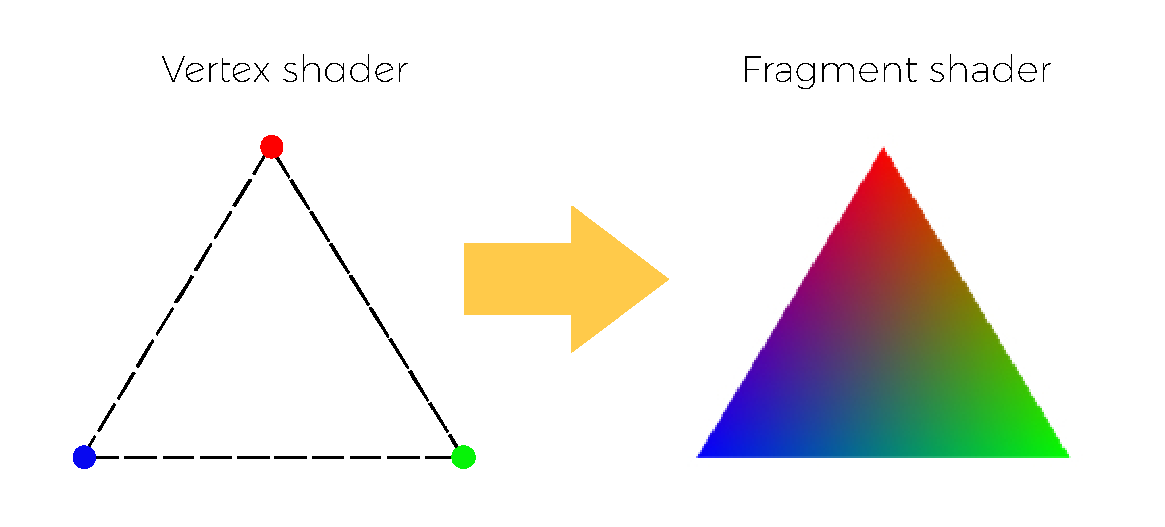
\includegraphics[scale=1.0,angle=0,width=1.0\linewidth]{obrazky-figures/interpolace}
	% 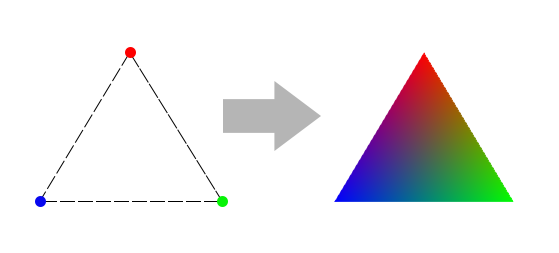
\includegraphics[scale=1.0,height=2.5in,angle=0]{obrazky-figures/interpolace.png}
	\caption{Ukázka interpolace hodnot mezi vertex a fragment shaderem.}
	\label{fig:inter}
\end{figure}
 



%=========================================================================
\newpage

\section{WebGL}
WebGL (\textbf{Web} \textbf{G}raphics \textbf{L}ibrary) je javascriptové aplikační rozhraní, které slouží pro nativní vykreslování 2D a 3D interaktivní grafiky přímo z webového prohlížeče \cite{mozilla}. K samotnému běhu WebGL není potřeba žádných dodatečných knihoven nebo zásuvných modulů, protože je v tomto ohledu využívána přímo grafická karta. Program WebGL se v zásadě skládá z více jazyků, přičemž každý mů svůj vlastní účel a je nutné je používat dohromady. Jedním z nich je javascript, druhý je jazyk GLSL. V jazyce GLSL jsou napsány dva programy - vertex shader a fragment shader. Oba programy kompiluje ovladač grafické karty do kódu, který je poté vykonáván přímo na grafické kartě. Vertex shader i fragment shader mohou být předávány jako řetězce, takže manipulace s nimi je díky tomu značně zjednodušena. Velkou výhodou WebGL je integrace s DOM tudíž od automatické správy pamětí přes zpracování událostí až po jednoduché načítání bitmapy přímo v prostředí prohlížeče apod. Zpracování všech dat i samotný běh programu je z hlediska implementace velice podobný konečnému automatu. 

K samotnému vykreslení je použit již výše zmíněný element HTML5 \texttt{<canvas>}, ze kterého se získá WebGL kontext.

V současné době je oficiálně vydána verze WebGL 1.0, která je založeno na OpenGL ES 2.0. Doposud se jedná o jedinou stabilní verzi. OpenGL ES\footnote{OpenGL for Embedded Systems.} je zjednodušená verze OpenGL, která eliminuje většinu vykreslovacích pipeline. Tato verze je především určena pro menší vestavěné systémy. Dalším rozšířením WebGL bude verze 2.0, která se stále nachází ve vývoji. Bude založena na OpenGL ES 3.0 přinášející velká vylepšení v zobrazování 3D grafiky - zejména textur, akceleraci vizuálních efektů, novou verzí jazyka GLSL s plnou podporu desetinných a celočíselných operací apod.



\subsection{Vykreslování primitiv}
K vykreslení nějakého grafického prvku jsou potřeba v zásadě jen dvě věci - vrcholy přepočítané do tzv. \textit{clipspace} a jemu přiřazené odpovídající barvy. Jak pro vrcholy, tak pro barvy slouží jiný GLSL shader. K vyobrazení objektu používá WebGL tří základní primitiva - vykreslení samotných bodů, čar nebo trojúhelníku. Vše funguje tak, že zadaný bod, kterému budeme chtít přiřadit barvu, se načte do odpovídající speciální globální proměnné ve vertex shaderu, kde se daná hodnota přepočítá do intervalu \texttt{<-1,1>} pro všechny jeho osy a vzniklá hodnota se uloží na grafické kartě. Počet bodu záleží na primitivu, které vykreslujeme. Pokud se tedy jedná o primitivum bodu, stačí pouze jeden bod ve vertex shaderu. V případě linky to bude dvojice bodů a u trojúhelníku trojice. GPU\footnote{Graphic Processing Unit - grafický procesor} poté zjistí, které pixely korespondují s vykreslovaným primitivem a pro každý takový pixel zavolá fragment shader. 


\subsection{Vyrovnávací paměť}
Buffery, resp. vyrovnávací paměti jsou rychle přístupné paměti na grafické kartě. V bufferech jsou  uloženy potřebná data k vykreslování grafických objektů jako např. body geometrie, normály, mapování textur aj. Data jsou poté dále předávány GLSL shaderům, které s nimi pracují.


%=========================================================================
\newpage

\subsection{Projekce}
Některé frameworky\footnote{Rámcová softwarová struktura usnadňující řešení dané problematiky} založené na WebGL zaměňují projekci za kameru, ta bohužel jako taková ve WebGL neexistuje. Jedná se pouze o způsob vykreslení grafické informace, ke které jsou využívány právě projekční zobrazení. WebGL podporuje dva základní typy projekce - ortografickou a perspektivní. 

Ortografická projekce využívá skutečné velikosti objektu. Scéna je reprezentována jako pravoúhlý hranol.

Perspektivní projekce zkresluje velikost objektů způsobem, jak je tomu v reálném světě. Čím je objekt dál od pozorovatele, tím se bude jevit jako menší, protože jeho pozice je středem této projekce. Dalším příkladem bychom mohli uvést koleje, které se v dálce jeví, jakoby se sbíhaly v jednu jedinou apod.
  
Pokud bychom chtěl vykreslit nějaký 3D objekt, bude potřeba mít v bufferech informace o vrcholech, normálách, textuře aj. Tyto data bychom zároveň museli neustále aktualizovat a nahrávat zpět do paměti, aby bylo možné s daným 3D objektem jakkoli manipulovat, posouvat atd., aby nedocházelo k neustálému přepisování hodnot v paměti na GPU. Veškeré změny zrealizujeme transformačními maticemi, kterými se bude geometrie objektu v paměti násobit, aniž by data v paměti byla jakkoli změněna.

\subsection{Homogenní souřadnice}
Homogenní souřadnice je tvořena čtyřmi prvky - \texttt{x}, \texttt{y}, \texttt{z} a \texttt{w}. První tři složky tvoří souřadnice euklidovského prostoru, poslední prvek \texttt{w} je perspektivní složka. Spolu se souřadnicemi \texttt{x}, \texttt{y}, \texttt{z} tvoří projekční prostor.\cite{WebGLbeg}

Perspektivním dělením, tedy vydělením souřadnic \texttt{(x, y, z)} perspektivní složkou \texttt{w}, lze získat normalizované hodnoty bodu zpět do trojrozměrného souřadného systému. Platí zde ale, že perspektivní složka nesmí být nulová. 

Samotná perspektivní složka funguje v homogenních souřadnicích jako změna měřítka daného bodu geometrie.

Jednou z dalších vlastností homogenní souřadnice je ta, že umožňuje definovat body do nekonečna, resp. nekonečnou délku vektoru, což ve standardním trojrozměrném prostoru možné není. Tato situace nastává v případě, kdy je složka rovna nule.

\subsection{Model matrix}
Jedná se o matici, kterou držíme pro každý vykreslovaný objekt. Stará se o úpravu tvaru, natočení a posuvu objektu.

\subsection{View matrix}
Díky takové transformační matici realizujeme již avizovanou \uv{roli kamery}, kdy simulujeme vzájemný vztah scény a pozorovatele.

\subsection{Perspective matrix}
Stará se o perspektivní zkreslení scény. Tato transformace rozhoduje o tom, jak velké zorné pole bude vykresleno a mapováno 
na obrazovku monitoru. \cite{zdrojak}

%=========================================================================
\newpage

\subsection{Vytvoření a běh programu}
Po vytvoření kontextu \texttt{webgl} je již možné využívat funkce pro práci v javascriptovém API. Funkce by se daly rozdělit na několik částí. Nejprve ty, které pracují s shadery, dále ty které vytváří program a v neposlední řadě funkce pro prací s buffery a vykreslením dat. Všechny funkce WebGL pracují nad vytvořeným kontextem plátna\footnote{Vytvořený WebGL kontext budeme označovat jako \texttt{gl}}. Práce s funkcemi WebGL je velice podobná konečnému automatu. V zásadě jde pouze o volání funkcí s danými parametry, které mění kontext pro specifické účely. WebGL disponuje celou řadou funkcí, které využijeme dále v implementaci. V této částí se ale zaměříme na vykreslování, které je třeba více popsat, než se vrhneme na samotnou implementaci. 

Po nahrání dat do bufferů se vykreslení uložených data realizuje funkcemi \texttt{drawArrays()} nebo \texttt{drawElements()}. Hlavní rozdíl mezi funkcemi je ten, že \texttt{drawArrays()} vykresluje přímo data geometrie tak,  jak byla spočítána a vložena do vertex bufferu. Samotné body prostoru, tak jak jsou definovány, jsou uvedeny vícekrát pro každé sousedící primitivum.

Funkce \texttt{drawElements()} pracuje s takovými daty odlišným způsobem. Vedle bufferů potřebných k vykreslení geometrie a mapování textury je zaveden nový buffer tzv. index buffer, který disponuje odkazy na jednotlivé body do bufferu geometrie a zavádí sdílení bodů, čímž data geometrie zmenší. 

 



%=========================================================================
\newpage

\chapter{Návrh klíčových částí prohlížeče}
\label{chapter:3}
Kapitola nastiňuje, jakým způsobem jsou řešeny nejzásadnější problémy implementace prohlížeče. Snaží se navrhnout ty nejefektivnější způsoby řešení daných problémů a v případě, že tomu tak v konkrétním případě není, snaží se tyto  kroky návrhu jasně odůvodnit, proč jsou  daným způsobem takto řešeny.


\section{Geometrie}
Geometrie je potřebná k mapování textury, a to tak, aby daná textura reflektovala scénu co nejvěrněji. Kdybychom pro texturu nevytvářeli geometrii, na kterou se bude mapovat a jednoduše data namapovali do libovolné 2D roviny, dojde k významnému zkreslení pořizované scény.

K uložení dat geometrie budeme využívat klasické pole, kde každý bod bude tvořen třemi rozměry v kartézské soustavě souřadnic o formátu \texttt{[x1,y1,z1, x2,y2,z2, … ]}, které utváří jednotlivé body v 3D prostoru. Body pak mezi sebou tvoří prostor, na který budou texturovací data  mapovaná. Ve WebGL jsme schopni vykreslit jednotlivé body, čáry – tedy spojnice jednotlivých bodů, nebo trojúhelníky. V našem případě bude potřeba vykreslit texturu jako plochu, na kterou se bude vše mapovat. Pro tento případ se ve WebGL používá renderování pomocí trojúhelníků jako základní vykreslované primitivum plochy.

Geometrickým tělesem pro mapování bude zvolena koule, protože scéna, resp. pořízená data, která budeme zpracovávat, jsou zachycena ve sférickém módu a mapováním na kouli je dosažena nejvěrnější reprezentace scény.

Kouli si rozdělíme na poledníky a rovnoběžky. Poledníkem je v tomto případě myšlena spojnice severního a jižního pólu, kde úhel z počátku kartézské soustavy souřadnic mezi jednotlivými poledníky nabývá hodnot od 0 do 360\degree. Rovnoběžkou je myšlena kružnice  rovnoběžná se vzájemně sousedícími a svírající úhel s počátkem souřadnic od 0 do 180\degree. 

Je třeba tedy nejprve stanovit počet poledníků a rovnoběžek a z takových hodnot bude dále vypočítán úhel. Na základě úhlu budeme schopni přesně definovat bod v trojrozměrné rovině. Čím větší počet rovnoběžek a poledníků, tím bude geometrie věrněji aproximovat kouli. Zároveň se ale zvýší hustota bodů v bufferech a tím bude i samotné vykreslení náročnější. Proto je ideální kompromis mezi jemností bodů a rychlosti načítání s téměř stejným výsledkem. Tato vlastnost by se nám hodila hlavně tedy v případech, kdy bychom měli vykreslit rozmanitý geometrický objekt se spoustou detailních sekvencí. V našem případě tento rozdíl nepůjde okem rozeznat, takže skrze efektivitu je výhodné spíše snížit počet rovnoběžek a poledníků, čímž dosáhneme pozitivního efektu na samotnou rychlost programu.


\subsection{Sférický souřadný systém}

Každá rovnoběžka má po svém obvodu průsečíky s jednotlivými poledníky. Tyto průsečíky jsou naše body geometrie, které budou nahrány do bufferů. Jelikož každá rovnoběžka nabývá úhlu od 0 do 180\degree,  resp. $0-\pi$, tak tento úhel můžeme podělit počtem rovnoběžek a vynásobit aktuální rovnoběžkou, čímž získáme svíraný úhel s počátkem souřadnic. Na obrázku \ref{fig:geom} označujeme tento úhel jako $\theta$. Provedením této operaci pro všechny horizontální obvodové kružnice vypočítáme všechny svírané úhly s počátkem souřadnic. 

Dále je nutné vypočítat svíraný úhel všech poledníků - vertikálních čar svírajících jej s počátkem souřadnic. Na obrázku \ref{fig:geom} je vyznačen jako $\varphi$. Jak jsem již nastínil výše, $\varphi$ nabývá hodnot od 0 do 360\degree, resp. $0-2\pi$. Vytyčený úhel mezi jednotlivými čarami jsme schopni spočítat tak, že jej podělíme počtem vertikálních čar a vynásobíme aktuálním poledníkem. Takto získáme rovnoměrné rozložení bodů na celé rovnoběžce. Provedením  operace pro všechny rovnoběžky již bude geometrie koule z hlediska úhlů kompletní.

\begin{figure}[h]
	\label{img:2}
	\centering
	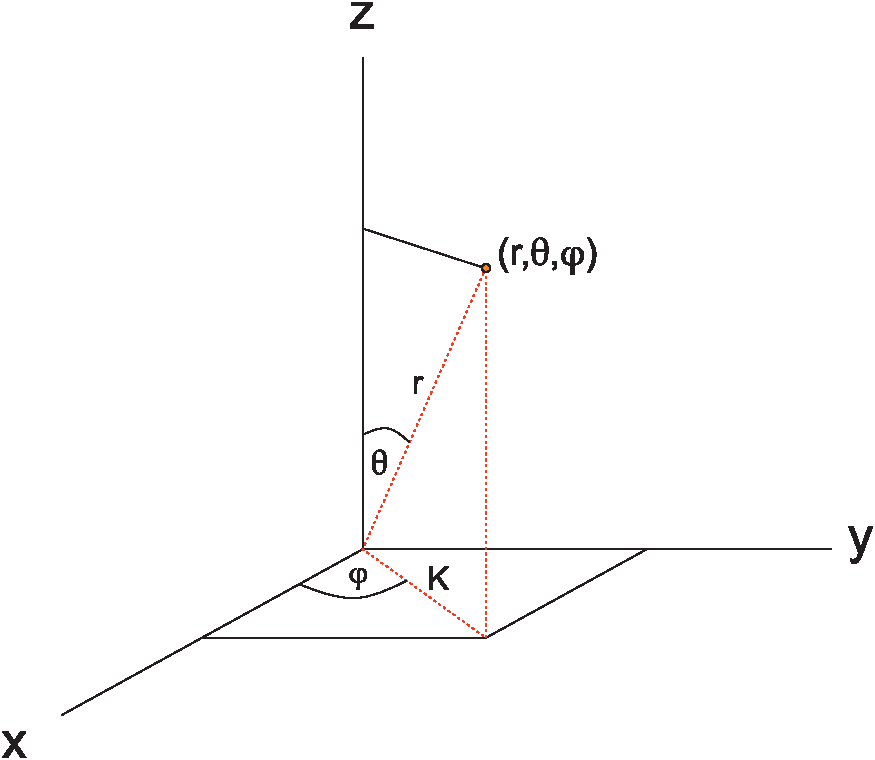
\includegraphics[scale=1.0,angle=0,width=0.6\linewidth]{obrazky-figures/geometry}
	\caption{Výpočet jednotlivých bodů geometrie}
	\label{fig:geom}
\end{figure}
 
Na základě vypočtených úhlů je možné již spočítat jednotlivé složky kartézské soustavy souřadnic \texttt{[x,y,z]} každému bodu, čímž dojde ke kompletní aproximaci tělesa.

%=========================================================================
\newpage

K výpočtu využijeme goniometrické funkce  a vztahy v pravoúhlém trojúhelníku. Jelikož $ \cos (\varphi) $ je dána poměrem délky přilehlé odvěsny a přeponou, tak souřadnici \texttt{\textit{x}} definujeme vtahem \cite{Goniometrie}:
 
\begin{equation}
 \cos (\varphi) = \frac{x}{K}  \Rightarrow x = \cos (\varphi) \cdot K
\end{equation}
\\
Ze vzniklého vztahu jasně vidíme, že je třeba dopočítat přeponu \textit{K} v trojúhelníku  o stranách $\arrowvert xKy\arrowvert$, kterou ale odvodíme vztahem odvěsny \textit{K} v trojúhelníku $\arrowvert zrK\arrowvert$. Mezi odvěsnou \texttt{K}\footnote{Z obrázku \ref{fig:geom} je patrné, že je přeponou v $\bigtriangleup xKy$, ale odvěsnou v $\bigtriangleup zrK$} a protilehlou přeponou \textit{r} platí, že délka odvěsny protilehlé k úhlu $\varphi$ a délka přepony mají vztah \cite{Goniometrie}:
\\
\begin{equation}
\label{math:K}
\sin (\theta) = \frac{K}{r}  \Rightarrow K = \sin (\theta) \cdot r
\end{equation}
\\
Všechny neznáme máme již dopočítané a můžeme dosadit do první rovnice, čímž dostáváme výsledný vztah převedené souřadnice z kartézské soustavy souřadnic do sférického souřadného systému:
\\
\begin{equation}
\label{math:x}
x = \sin (\theta) \cdot  \cos (\varphi) \cdot r
\end{equation}
\\
Následující souřadnici \texttt{y} vyjádříme obdobným vztahem jako u předchozí souřadnice, ale s tím rozdílem, že protilehlá odvěsna bude k úhlu $\varphi$ a přeponou bude strana \texttt{K}:
\\
\begin{displaymath}
\sin (\varphi) = \frac{y}{K}  \Rightarrow y = \sin (\varphi) \cdot K
\end{displaymath}
\\
Opět máme v rovnici pro výpočet souřadnice \texttt{y} stranu \texttt{K}, kterou ale máme již vypočtenou ve vztahu \ref{math:K}, tudíž už jen tento vztah dosadíme a vznikne výsledná rovnice hledané  souřadnice:
\\
\begin{equation}
\label{math:y}
y = \sin (\varphi) \cdot \sin (\theta) \cdot r
\end{equation}
\\
Poslední souřadnice \texttt{z} je značně jednodušší, protože nám odpadá proměnná \texttt{K}. Vyjádření souřadnice \texttt{z} je principiálně úplně stejné, jako tomu bylo u souřadnice \texttt{x} - přilehlá odvěsna k úhlu $\varphi$ ku přeponě \texttt{r}. Výsledný vztah je tedy možné vyjádřit následovně:
\\
\begin{equation}
\label{math:z}
\cos (\theta) = \frac{z}{r} \Rightarrow z = \cos (\theta) \cdot r
\end{equation}

%=========================================================================
\newpage


\subsection{Vrcholy}
Jakmile máme vypočítány konkrétní složky trojrozměrného prostoru - tedy kompletně spočtený sférický souřadný systém, můžeme přistoupit ke kompletaci dat určených k nahrání do grafické karty. Těmito daty jsou vrcholy samotné geometrie, texturovací data a indexy. 

Získání samotného vrcholu lze vynásobením složek \texttt{x}, \texttt{y} a \texttt{z} průměrem tělesa \texttt{r}. Tato operace musí být provedena u všech bodů koule.

Vzniklé těleso vyobrazené pomocí čar\footnote{Použito grafické primitivum \texttt{gl.LINES}.} je demonstrováno na obr. \ref{img:3}.


\begin{figure}[h]
	\label{img:3}
	\centering
	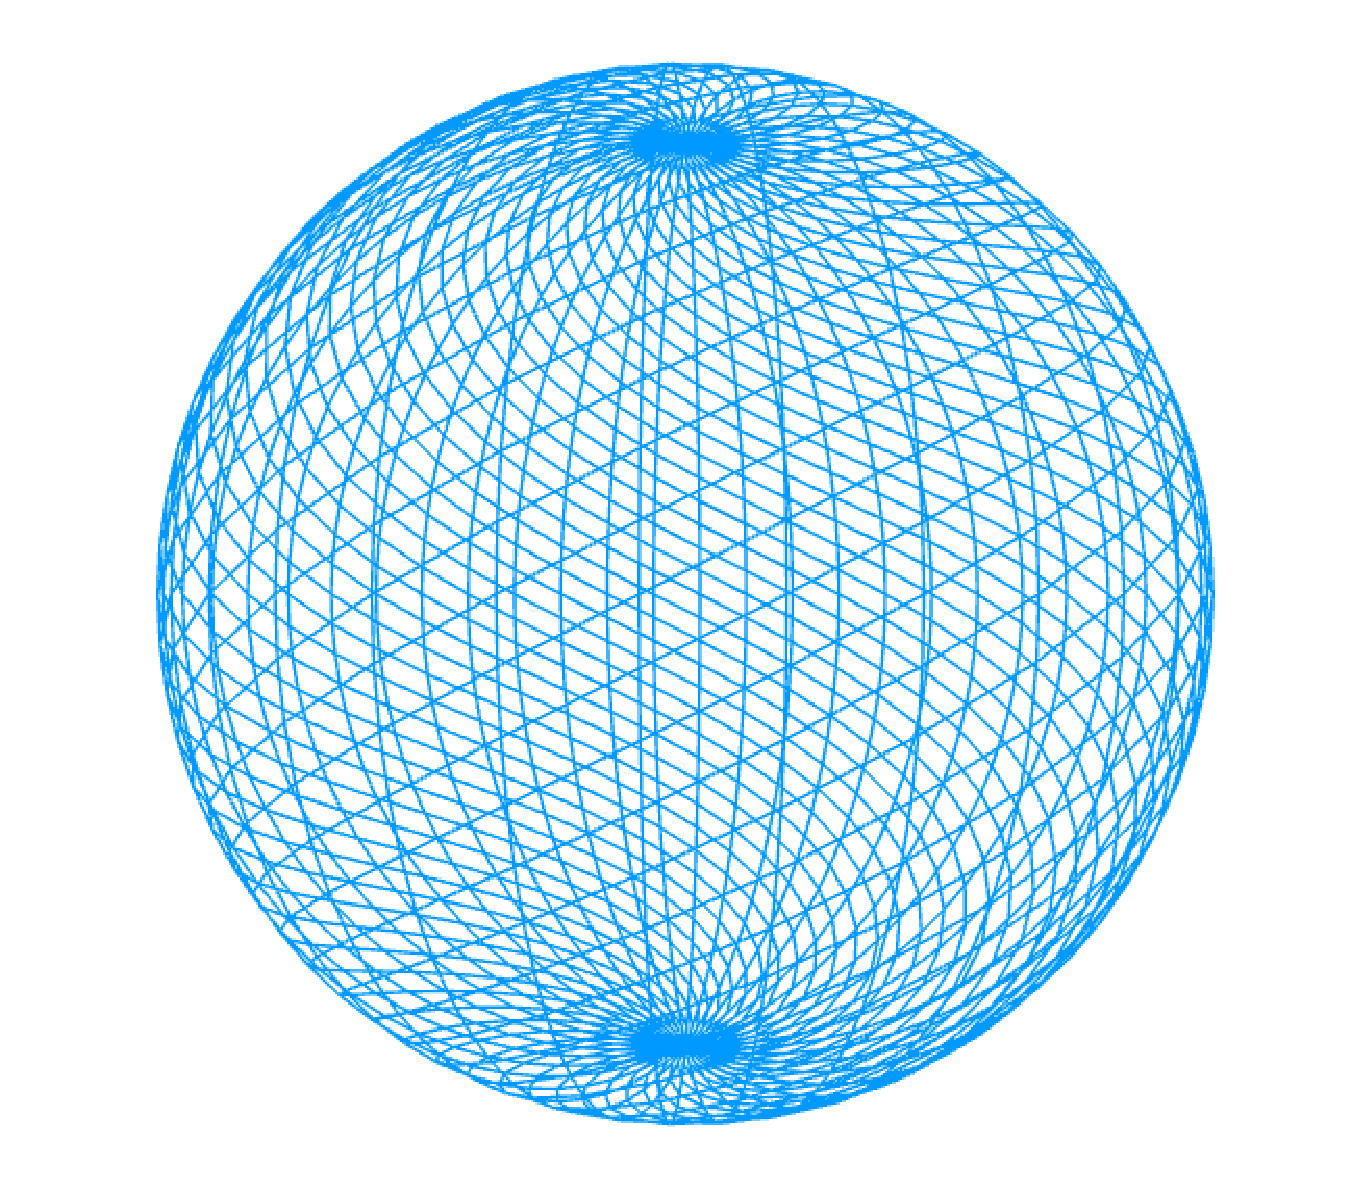
\includegraphics[scale=1.0,angle=0,width=0.55\linewidth]{obrazky-figures/vertex}
	\caption{Koule vyobrazena pomocí čar}
	\label{fig:geom2}
\end{figure}


\subsection{Textura}
Data textury se počítají oproti vrcholům zcela odlišně. Všechny body textur jsou v současné stabilní verzi WebGL pouze dvojrozměrné, tudíž souřadnice \texttt{z} nebudeme potřebovat.
Počet bodů textury bude přímo záviset na počtu rovnoběžek a poledníků.

Od zvoleného počtu rovnoběžek a poledníků se bude dále odvíjet počet bodů textury tak, že pro každou rovnoběžku se spočítají všechny poledníky. Celkový počet bodů textury bude roven: \textit{počet\_rovnoběžek $\cdot$ počet\_poledníků}.

%=========================================================================
\newpage

Pro lepší představu mapovaní textury můžeme jak poledníky, tak rovnoběžky znázornit ve dvourozměrném prostoru, kde jednotlivé průsečíky tvoří body textury. Horizontální čáry prezentují souřadnici s označením \texttt{\textbf{u}}. Vertikální čáry zase souřadnici \texttt{\textbf{v}}. 

Znázornění demonstruje obrázek \ref{img:grid}. Souřadnici \texttt{\textbf{u}} spočteme vydělením \textit{k}-tého poledníku celkovým počtem poledníků. Souřadnici \texttt{\textbf{v}} zase vydělením \textit{k}-té rovnoběžky celkovým počtem rovnoběžek.

\begin{figure}[h]
	\label{img:grid}
	\centering
	
\includegraphics[scale=1.0,angle=0,width=0.35\linewidth]{obrazky-figures/grid}
	\caption{Mapování textury}
\end{figure}

\subsection*{Výpočet konečné barvy ve fragment shaderu}
Výsledná interpolovaná barva textury se ve fragment shaderu vypočítá vztahem:

$$ gl\_FragColor = t(s, v_{t}) $$ 

kde \texttt{t} je texturovací funkce, která načte data fragmentu, \texttt{s} označuje vzorkovací proměnnou a $v_{t}$ interpolovaný bod z vertex shaderu.


\subsection{Indexy}
Zavádění indexů se vyplatí tehdy, pokud chceme vykreslování objektu zefektivnit z hlediska vykreslování jednotlivých bodů. V případě, že se při vykreslování nepoužívá index buffer, tak se pro každé vykreslované primitivum načítá adekvátní počet vrcholů. Potíž nastává v situaci, kdy je vrcholy společný. Dojde k tomu, že souřadnice vrcholu jednoho bodu bude v paměti vícekrát a bude volán pro každé primitivum zvlášť. Díky indexům je pro danou geometrii zmíněn sdílený bod právě jednou. V index bufferu je tento bod zmíněn vícekrát, ale odpovídá mu právě jeden bod geometrie. Díky tomuto odkazování se nám sníží počet vykreslovaných bodů. Indexování se používá spolu s funkcí \texttt{drawElements()} a pro účely implementace bude využita pro zrychlení načítání ekvidistantního zobrazení textur.

%=========================================================================
\newpage

\subsubsection{Návrh index bufferu}
Rovnoběžky a poledníky využijeme i v této části. Jak lze z obrázku \ref{img:grid} pozorovat, horizontální a vertikální čáry tvoří mezi sebou čtvercovou síť, kdy čtverec můžeme snadno interpretovat pomocí trojúhelníku jako grafického vykreslujícího primitiva víz obr. \ref{img:indexes}.



\begin{figure}[h]
	\label{img:indexes}
	\centering
	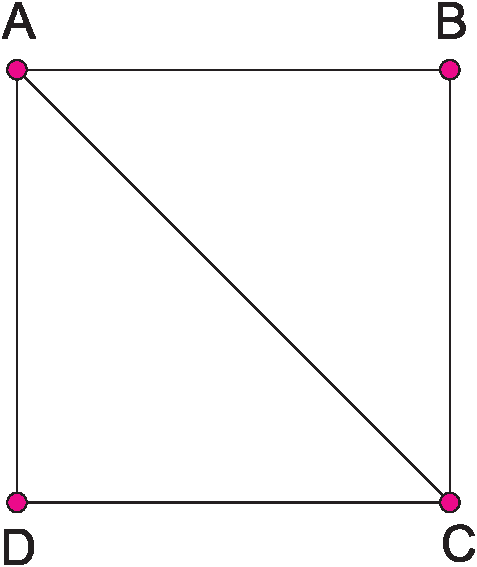
\includegraphics[scale=1.0,angle=0,width=0.5\linewidth]{obrazky-figures/indexes}
	\caption{Implementace indexů}
\end{figure}

Je tedy jasně patrné, že čtverec budeme vykreslovat trojúhelníky $ABC$ a $ADC$. Horizontální přímky protínající body \textit{A}, \textit{B} a \textit{D}, \textit{C}   jsou rovnoběžky, po kterých se budeme při výpočtu bodů posouvat. Naproti tomu body \textit{A},\textit{D} a \textit{B}, \textit{C} prochází poledníky, díky kterým budeme při výpočtu realizovat vertikální posuv.

Samotné zpracování indexů tedy probíhá tak, že pro každou rovnoběžku procházíme její průsečíky s danými poledníky. Do index bufferu uložíme pro každé grafické primitivum trojici bodů, což tedy v praxi znamená šestici bodů pro každý čtverec sítě, kde se budou vždy dva body opakovat.

%=========================================================================
\newpage

\section{Korekce textur}
Základní mapování textury lze pozorovat na obr. \ref{img:grid}. Takové mapování lze využít u equirectangulárního prohlížení, kde samotná vstupní textura má jíž vše potřebné a není tedy již potřeba nic upravovat - samotná ekvidistantní projekce již je převod tělesa trojrozměrného zobrazení do 2D, proto přímo koreluje s daty textury. Pro režim rybího oka je situace složitější, protože vstupní textura není v equirectangulárním módu, a naším úkolem je udělat korekci textury tak, aby se textura namapovala na kouli co nejpřesněji.


\begin{figure}[h]
	\label{img:texture_without_correction}
	\centering
	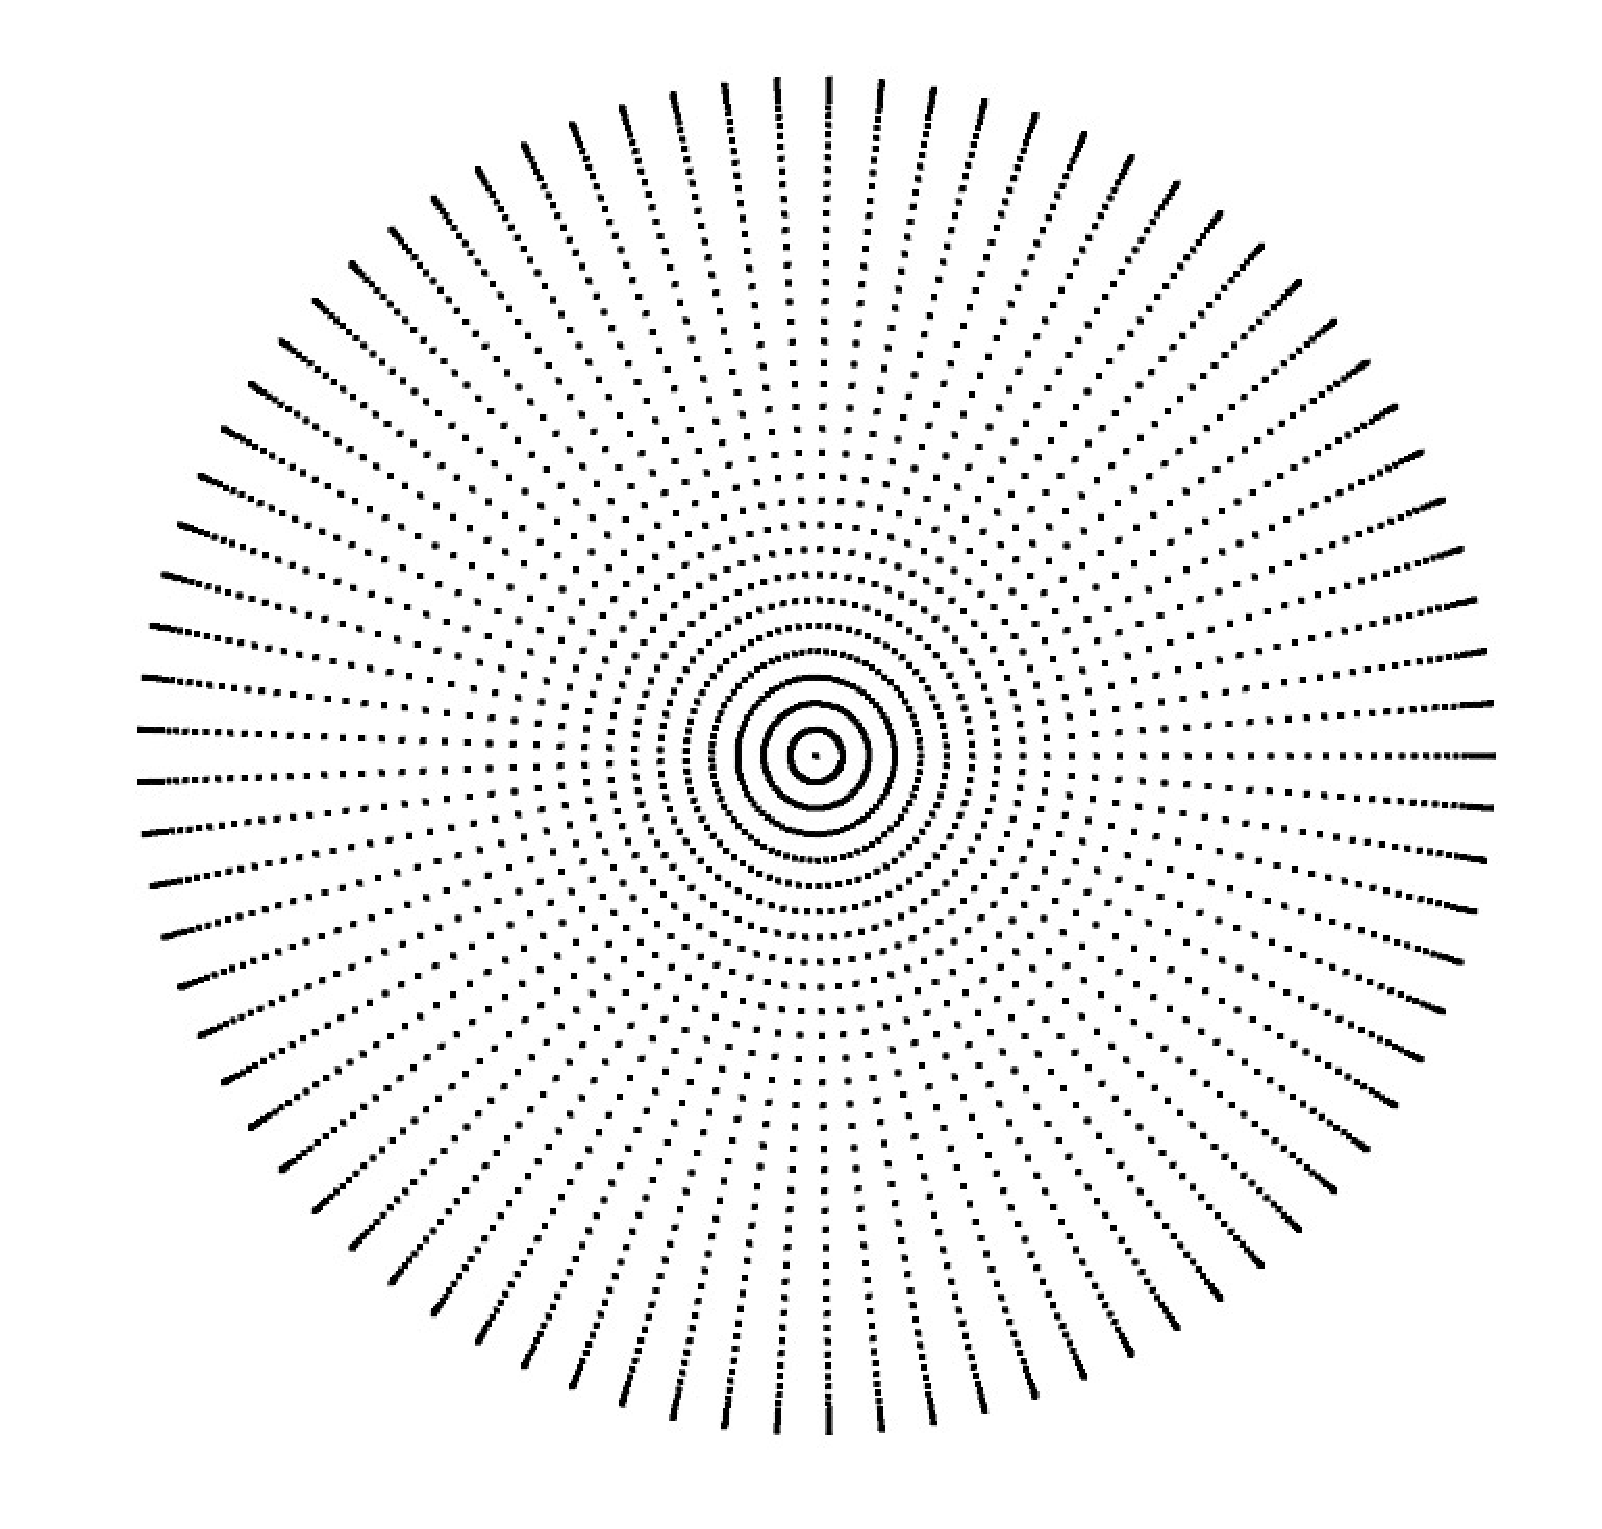
\includegraphics[scale=1.0,angle=0,width=0.6\linewidth]{obrazky-figures/texture}
	\caption{Textura vycházející z předpočítaných dat. Bez korekce.}
\end{figure}

\section{Korekce pro rybí oko}
Korekci využijeme především k tomu, aby se nám textura mapovala přesněji v oblasti švu, tedy přesně v polovině tělesa. Důvodem je ten, že pokud bychom korekci textury neudělali, okraje by byly rozostřené  a v oblasti švu data hůře čitelná.  Samotná korekce nemá na funkci prohlížení žádný vliv.
S korekcí se mapuje textura daleko přesněji, resp. okraje hemisféry. Na obrázku \ref{img:texture_without_correction} si lze povšimnout ukázky dat textury ještě před provedením korekce krajních bodů.

Pro výpočet korekce můžeme využít jako počáteční hodnoty souřadnic již ty spočítané pro normály\footnote{V našem případě hodnota souřadnice vrcholu podělená průměrem tělesa.}, popř. vrcholy geometrie.

Již před-počítané hodnoty je ale nutné ještě upravit, protože jsou počítány pro trojrozměrný prostor a my pro texturu potřebujeme pouze dva rozměry. Úpravou je v tomto smyslu myšleno to, že velikost poloměru  kružnice se bude měnit rovnoměrně. Hlavně tedy u bodů, které odpovídají těm v oblasti švu. V tomto místě dochází k největšímu zhuštění bodů, což má za následek již avizované neúměrné roztažení a deformaci textury.

%=========================================================================
\newpage




Je-li  souřadnice \textit{\textbf{\axisY}} definována rovnicí \ref{math:\axisY} a souřadnice \textit{\textbf{\axisZ}} vztahem \ref{math:\axisZ}, tak korekce textury bude realizována vynásobením  vertikální a horizontální souřadnice funkcí \textit{\textbf{arccos(\axisY)}}. Každá hemisféra koule bude mít odlišnou modifikaci souřadnice \texttt{\textbf{\axisX{}}}, protože výpočet každé hemisféry probíhá v jiném kvadrantu kartézské soustavy souřadnic. V opačném případě bychom nemohli mapovat obě sféry z důvodu, že by se nám spojily do jedné tj. body by se překrývaly. Důvod je zřejmý, data z kterých korekce vychází jsou počítány pro celou kouli a nerespektováním změny souřadnice by se bod zobrazil až  \uv{za} vyobrazeným bodem na obrazovce\footnote{Z pohledu na těleso ve 3D.}. \\

Horizontální a vertikální souřadnici \texttt{\textbf{u}} a \texttt{\textbf{v}} spočítáme následujícím způsobem:




\begin{itemize}
	\item Pro levou hemisféru bude platit následující vztah:\\
		    $$u =  \axisX{} \cdot \frac{\arccos(\axisY{})}{r} \wedge v =  \axisZ{} \cdot \frac{\arccos(\axisY{})}{r}$$   
		   
	\item Pravá hemisféra je definována vztahem:\\
			$$u =  -\axisX{} \cdot \frac{\arccos(\axisY{})}{r}\wedge v =  \axisZ{} \cdot \frac{\arccos(\axisY{})}{r} $$ 
 
\end{itemize}
 

\begin{figure}[h]
	\label{img:texture_with_correction}
	\centering
	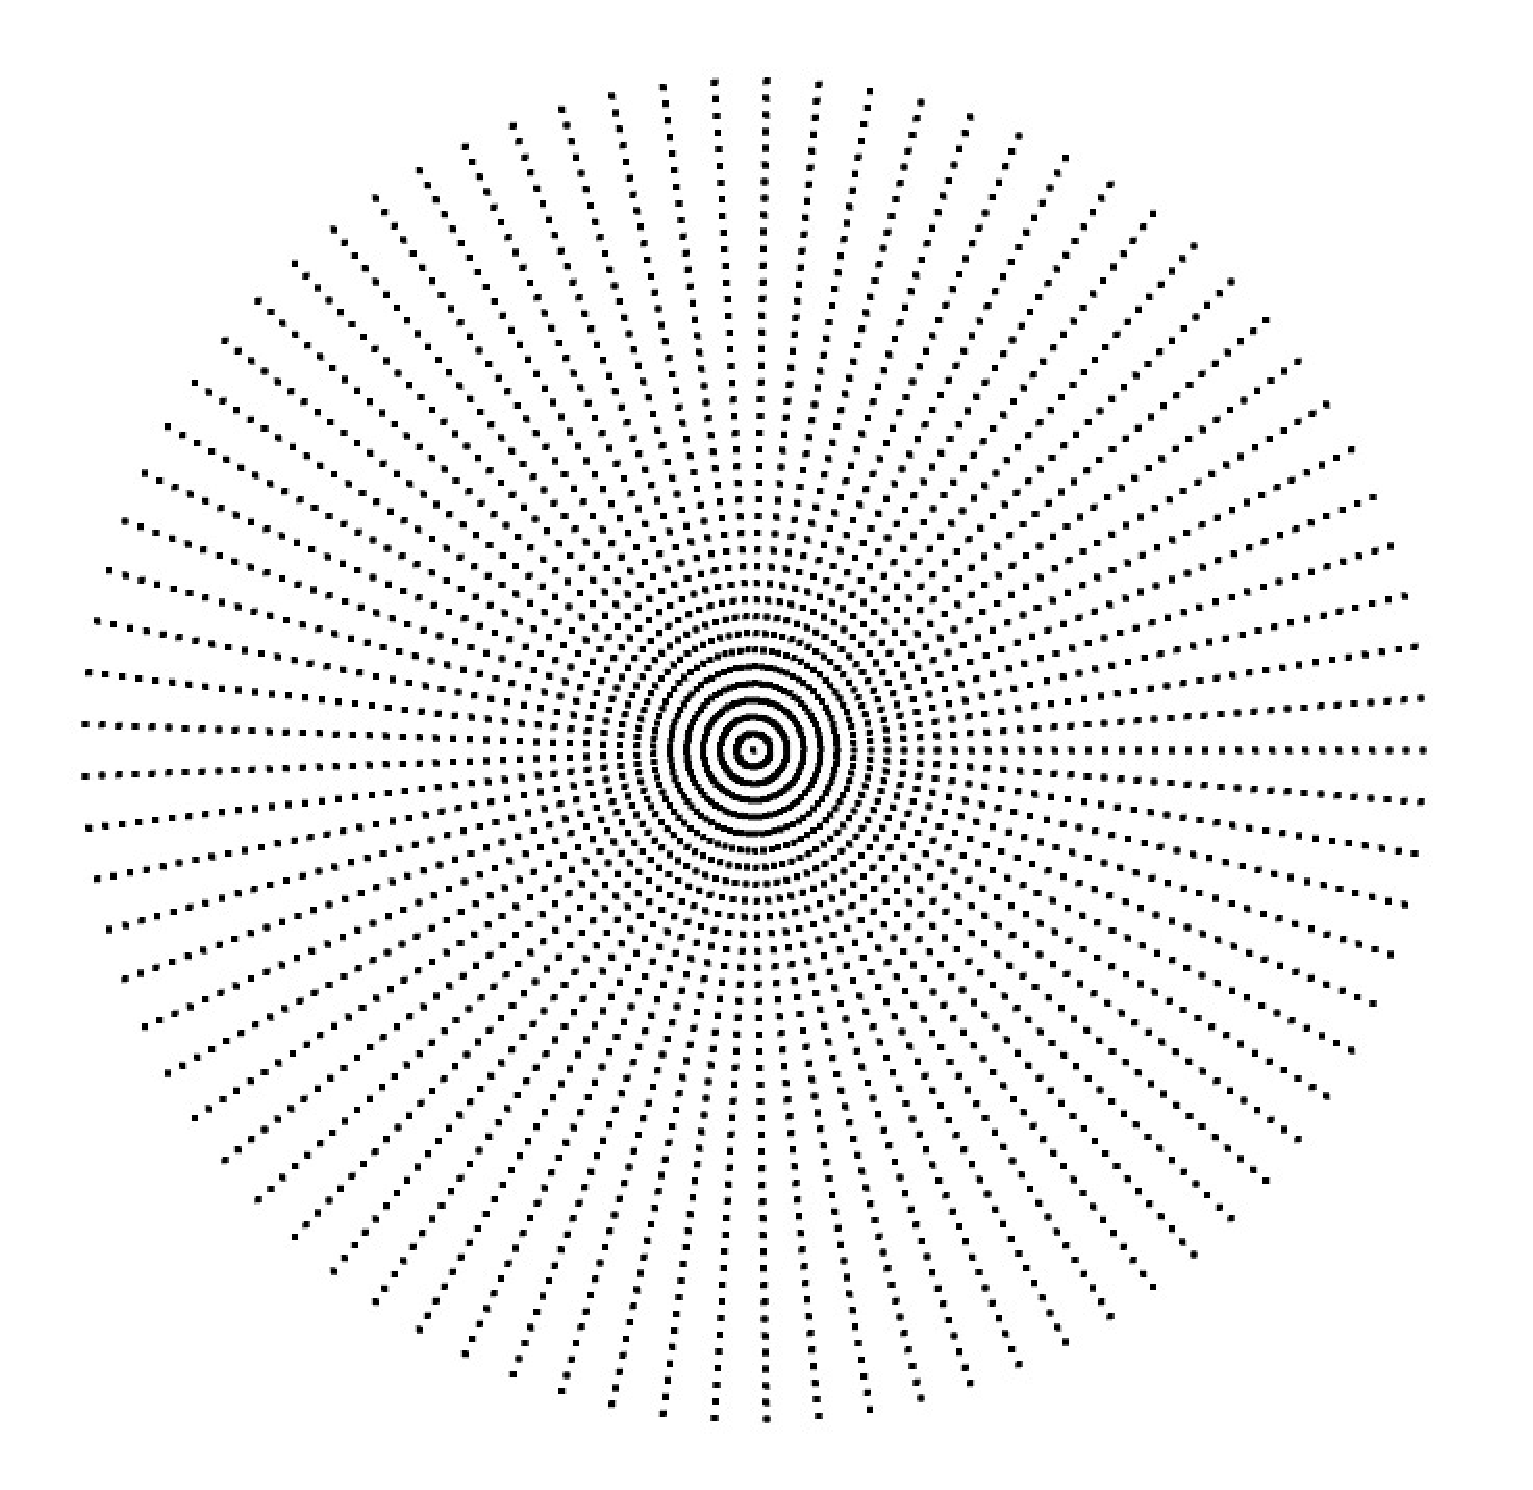
\includegraphics[scale=1.0,angle=0,width=0.6\linewidth]{obrazky-figures/texture_correction}
	\caption{Textura s korekcí krajních bodů.}
\end{figure}

Proměnná \texttt{r} označuje poloměr koule, resp. kružnice ve 2D. Obrázek \ref{img:texture_with_correction} demonstruje již aplikovanou  korekci vstupních dat  textury z obr. \ref{img:texture_without_correction} avizovanou výše.
 

%=========================================================================
\newpage


\section{Návrh projekce}
Součástí již zmíněné projekce v předchozí kapitole jsou matice, které modelovou, zobrazovací a projekční matici utváří. Mezi ně patří např. rotační matice po osách \texttt{x},\texttt{y} a \texttt{z}, dále matice posuvu, změny měřítka aj. Díky maticím jsme schopni projekci zrealizovat. V perspektivním pojetí vyváříme frustrum\footnote{V ortografickém zobrazení by to byl kvádr/krychle.}, resp. komolý jehlan, kdy stěny tvoří lichoběžník a obě podstavy čtverec. Veškeré vykreslovaná data, která neleží v komolém jehlanu jsou ořezány  a nebudou vykreslena. 




\subsection{Modelová matice}
Sem patři rotační matice všech os souřadného systému, dále matice pro změnu měřítka souřadnic a posuvná matice objektu.

Cílem modelové matice je tedy transformovat body modelu ze středu souřadného systému, vůči kterému byly body geometrie modelu napočítány, do zobrazitelného prostoru, se kterým budeme dále pracovat. Cílem modelové matice je posunout a pootočit zobrazovaným objektem do výchozí pozice promítání. Otáčení a další operace v reálném čase jsou  doménou zobrazovací matice. Začneme s matici pro změnu měřítka modelu:

$$
S =
\begin{pmatrix} 
\textbf{x} & 0 & 0 & 0\\
0 & \textbf{y} & 0 & 0\\ 
0 & 0 & \textbf{z} & 0\\ 
0 & 0 & 0 & 1\\ 
\end{pmatrix}$$

Dalšími operacemi je otočení kolem os \texttt{x}, \texttt{y} a \texttt{z}. Jedná se o typ shodného zobrazení, při kterém se těleso otočí o tzv. \textit{úhel otočení} kolem pevného bodu. \cite{Kompendium}
\newline


Matice rotace kolem osy \texttt{x}:

$$
R_{x}=
\begin{pmatrix} 
	1 & 0 & 0 & 0\\
	0 & \cos(\alpha) & -\sin(\alpha) & 0\\ 
	0 & \sin(\alpha) & \cos(\alpha) & 0\\ 
	0 & 0 & 0 & 1\\ 
\end{pmatrix}$$

Matice rotace kolem osy \texttt{y}:

$$
R_{y}=
\begin{pmatrix} 
 \cos(\alpha) & 0 & \sin(\alpha) & 0\\
0 & 1 & 0 & 0\\ 
-\sin(\alpha) & 0 & \cos(\alpha) & 0\\ 
0 & 0 & 0 & 1\\ 
\end{pmatrix}$$

Matice rotace kolem osy \texttt{z}:

$$
R_{z}=
\begin{pmatrix} 
\cos(\alpha) & -\sin(\alpha) & 0 & 0\\
\sin(\alpha) & \cos(\alpha) & 0 & 0\\ 
0 & 0 & 1 & 0\\ 
0 & 0 & 0 & 1\\ 
\end{pmatrix}$$

%=========================================================================
\newpage


Translační matice posunu objektu po osách \texttt{x},\texttt{y} a \texttt{z}\footnote{Druhou variantou matice je prohození \texttt{x},\texttt{y} a \texttt{z}  namísto nul ve čtvrtém sloupci prvního až třetího řádku.}. Přímo vychází z identické matice\footnote{Obsahuje na hlavní diagonále pouze jedničky. Všechny ostatní hodnoty jsou nulové.}:


$$
T =
\begin{pmatrix} 
1 & 0 & 0 & 0\\
0 & 1 & 0 & 0\\ 
0 & 0 & 1 & 0\\ 
\textbf{x} & \textbf{y} & \textbf{z} & 1\\ 
\end{pmatrix}$$



Výsledná modelová matice \texttt{\textbf{M}} je tedy dána vztahem:
$$ M = T \cdot R_{x} \cdot R_{y} \cdot R_{z} \cdot S $$

Při násobení původní matice rotačními maticemi hrají  velkou roli také znaménka. Jelikož v implementační části budeme používat interakce s myší a tím měnit náhled pozorovatele, resp. kamery na náš model, bude třeba zvolit směr posuvu zorného pole kamery. 

Vlastnosti prohození znamének využijeme právě u  rotace $R_{x}$ a $R_{y}$, které reprezentují pohyb myši.  


\subsection{Zobrazovací matice}
Jedná se o matici, která kontroluje způsob, jakým se na objekt díváme. V našem konkrétním případě budeme zobrazovací matici používat k napodobení pohybu kamery snímající objekt, jak je tomu v reálném světě. 

Prostor objektu, který jsme pomocí modelové matice transformovali do zobrazitelného prostoru, musíme nyní převést do prostoru, který bude relativní vzhledem k pohledu pozorovatele.

Takového efektu docílíme tak, že složku o kterou se chceme posunout vynásobíme opačnou hodnotou modelu ve scéně. Výsledný vztah pro výpočet zobrazovací matice tedy je \cite{WebGLbeg}:

$$ V = T \cdot R_{x} \cdot R_{y} \cdot R_{z} $$ 

%=========================================================================
\newpage


\subsection{Perspektivní matice}
Poslední častí projekce je perspektivní matice, díky které budeme realizovat zkreslení scény. Mezi vstupní parametry patří úhel neboli zorné pole. Čím by bylo zorné pole blíže hodnotě $\pi$, resp. \texttt{180\degree}, tím by se předmět v zorném poli jevil dál od pozorovatele. \cite{webglFUND} Hodnota \texttt{180\degree} je krajní hodnota zorného pole. Pokud bychom se jí příliš přibližovali, tak by se nám projekční prostor více a více zmenšoval, až by se objekt jevil nekonečně daleko a tedy se vůbec nezobrazil, protože v přímém úhlu je projekční plocha nulová.  Naopak zmenšováním hodnoty by se objekt jevil zase blíže. Zorné pole budeme označovat jako \texttt{\textit{fov}}. Bližší hranici projekčního prostoru jako \texttt{\textit{near}}, vzdálenější hranici jako \texttt{\textit{far}}.



\begin{figure}[h]
	\label{img:perspective_matrix}
	\centering
	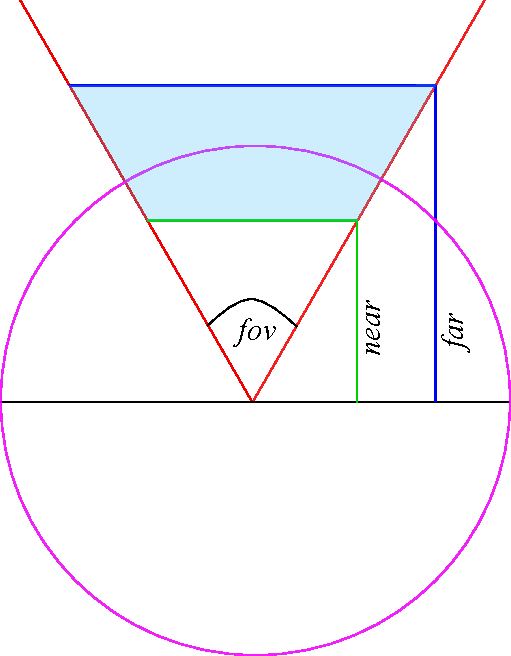
\includegraphics[scale=1.0,angle=0,width=0.45\linewidth]{obrazky-figures/perspective_matrix}
	\caption{Demonstrace perspektivního zobrazení.}
\end{figure}

Perspektivu demonstruje obrázek \ref{img:perspective_matrix}. Modře vyznačená plocha reprezentuje již zmíněný projekční prostor, který je definován  zorným úhlem a hranicemi. Fialová kružnice značí data textury, která se mapují na vypočítanou geometrii.

%=========================================================================
\newpage

Jednotlivé vstupní argumenty potřebné pro výpočet perspektivní matice zobrazení:

\begin{description}
		\item[fov] - pole, které definuje zorný úhel
		\item[aspect] - poměr šířky a výšky scény
		\item[near] - reprezentuje rovinu, která ořeže tu část modelu, která je příliš blízko pozorovateli
		\item[far] - reprezentuje rovinu, která ořeže tu část modelu, která je příliš daleko pozorovateli
\end{description}


$$
P =
\begin{pmatrix} 
\dfrac{1}{aspect \cdot \tan\left(\dfrac{ fov }{2}\right)} & 0 & 0 & 0\\
0 & \dfrac{1}{\tan\left(\dfrac{ fov }{2}\right)} & 0 & 0\\ 
0 & 0 & \left(\dfrac{near+far}{near-far}\right) & -1\\ 
0 & 0 &  \left(\dfrac{near \cdot far \cdot 2}{near-far}\right)  & 1\\ 
\end{pmatrix}
$$



\section{Výpočet projekce}
Konečný  vztah pro výpočet projekce scény $P_{s}$ bude dán pouhým vynásobením spočtených matic v následujícím pořadí:
$$ P_{s} = P \cdot V \cdot M  $$

 
vypočítaná projekce se poté násobí bodem geometrie $G$. Výsledná pozice bodu ve vertex shaderu má proto   vztah:

$$ gl\_Position  = P_{s} \cdot G$$

%=========================================================================
\newpage

\section{Zorný úhel}
Zorný úhel je grafický prvek, který udává informace o aktuálním zorném poli  perspektivní matice ve vztahu k zobrazovací matici. Jeho hodnota se mění na základě přibližování nebo oddalování scény od pozorovatele. 


\subsection{Vztah perspektivy a pozorovatele}
Základem pro výpočet zorného úhlu je perspektivní matice - přesněji argument \texttt{\textit{fov}}, který značí již výše zmíněné horizontální zorné pole. Celý výpočet bude  založen na axiomu o středovém úhlu, pro který platí, že je dvojnásobkem úhlu středového.\cite{planimetrie} 

Jedinou neznámou je v takovém případě právě středový úhel, který bude reprezentovat velikost zorného pole.

K odvození zorného úhlu na základě přiblížení scény je nutné spočítat \textbf{extrémy úhlů}. Na obrázku \ref{img:field_vision_implementation} tyto extrémy značí modrý a žlutý bod. Pokud vypočteme úhel pro každý z daných bodů, lze jej pak díky poměru přiblížení scény již snáze dopočítat. Na obrázku níže lze vidět kružnice \texttt{\textit{m}} a \texttt{\textit{t}}. Vnější fialová kružnice \texttt{\textit{t}} značí texturu, zelená čárkovaná  s označením \texttt{\textit{m}} zase maximální meze přiblížení. Z obrázku lze pozorovat, že $ \alpha = fov$, tudíž zorný uhel ve žlutém dolním extrému $E_{l}$ je roven: $$ E_{l} = 2 \cdot \alpha \cdot M_{l} $$

kde $M_{l}$ je zmenšení, aby extrém ležel na kružnici \texttt{\textit{m}}. Pro modrý extrém $E_{h}$ potom bude platit vztah\footnote{Kdyby $M_{h}$ nebyl definován, tak by extrém $E_{h}$ byl roven \texttt{0}\degree a pozorovatel by byl na hranici scény.}: $$ E_{h} = \alpha \cdot M_{h} $$


\begin{figure}[h]
	\label{img:field_vision_implementation}
	\centering
	\includegraphics[scale=1.0,angle=0,width=0.45\linewidth]{obrazky-figures/field_vision_implementation}
	\caption{Textura s korekcí krajních bodů.}
\end{figure}


%=========================================================================
\newpage

\subsection{Návrh prvku}
K realizaci prvku budeme potřebovat vektor \textbf{svg} zobrazující přímý úhel. Reprezentován bude tvarem polokoule, u které se využije vlastnosti tahu. Ve vektorové grafice se jedná o nastavení atributu \texttt{stroke-width}, který bude znázorňovat zorný úhel. Důvodem, proč pro vyobrazení  není využita samotná křivka vyplněná barvou, je ten, že pokud se přenastaví úhel zobrazení, tak se křivka zdeformuje způsobem, že z ní zorný úhel není zjevný.

Vstupními argumenty je pozice prvku ve dvojrozměrném prostoru \texttt{(x,y)} a průměr kruhu. Dále je potřeba přepočítat tyto souřadnice dvojrozměrného prostoru na polární souřadnice. K samotnému výpočtu dostačuje Pythagorova věta, kdy pomocí bodu \texttt{(x,y)} jsou známy hodnoty odvěsen a je možné spočítat přeponu. \cite{geometrie} Takto odvodíme vztahy \\pro \texttt{x} a \texttt{y}.


 $$ x = r\cdot\cos(\theta) $$ 
 $$ y = r\cdot\sin(\theta) $$  






%=========================================================================
\newpage


\section{Kompas}
Dalším rozšířením prohlížení jsou údaje o světových stranách díky kompasu. Střelka kompasu se bude pohybovat k severu díky vstupním argumentům, které budou předány přímo do programu. Ukazatel severu se bude měnit na základě rozdílu vůči vstupní pozici, která definuje pozici severu ve scéně. Střelka bude realizována obrázkem, a její natočení pomocí změny kaskádových stylů, která bude udávána ve stupních vůči původní pozici. Samotná transformace zobrazení, resp. otočení střelky budeme realizovat pomocí vlastnosti kaskádových stylů \texttt{transform: rotate(\textbf{\emph{X}}deg)} kde \texttt{\textbf{\emph{X}}} je posuv ve stupních.

\subsection{Odchylka střelky}
Korekce kompasu bude daná úhlem, který svírá střed zorného pole se vstupní statickou pozici zadanou argumentem programu. Statická pozice zůstává po celou dobu běhu programu neměnná. Samotná korekce bude reagovat pouze na změnu horizontální osy.

\subsection{Výpočet pozice kompasu v plátně}
Výsledné zobrazení kompasu, resp. jeho pozice, je přímo závislá na rozměrech elementu \texttt{<canvas>}. Je to z toho důvodu, že prvek plátno překrývá. Samotný výpočet a následné korekce změnou šířky plátna, popř. využití režimu celé obrazovky vyžaduje přepočítání pozice, která je definována vztahem:

$$ \left( Canvas_{width} - Compass_{width}\right) \cdot x  $$
$$ \left( Canvas_{height} - Compass_{height}\right) \cdot y  $$

kde $Canvas_{width}$ a $Canvas_{height}$ jsou vstupní argumenty kompasu udávající velikost prvku. Naproti tomu  $x$ a $y$ souřadnice nabývající hodnot od $0$ do $1$, která definuje pozici v plátně nezávisle na rozlišení.

%\section{Metadata}
%\section{Blending}
%=========================================================================

\chapter{Implementace panoramatického prohlížeče}
\label{chapter:4}
V této kapitole rozeberu implementaci programu  spolu s  problémy, které bylo nutné v průběhu implementace řešit. Program se skládá z jazyka HTML5, ve kterém je nastíněna výchozí kostra, nad kterou pracuje veškerá funkcionalita. Jádro je napsáno v jazyce Javascript bez použití frameworků  a  dále shadery, které jsou implementovány v jazyce GLSL. 


\section{Stavy a data programu}
Jelikož samotná implementace ve WebGL vyžaduje k realizaci problematiky více jazyků, vzniká v programu velké množství proměnných, které je velice vhodné určitým způsobem pro vyšší přehlednost v kódu sdružovat. Program jako takový je napsán procedurálním stylem, ale sám využívá některé objektové vlastnosti. Mezi ně patří právě sdružování proměnných, které jsou hierarchicky uspořádány do objektu.

Každá důležitá část implementace má svůj vlastní objekt proměnných, které se k dané problematice vztahují, včetně všech nutných interních stavů.

\subsection{Myš a klávesnice}
Veškeré interakce s myší se z hlediska datové částí promítají do objektové proměnné \texttt{MOUSE}, která udržuje data o pohybu pozorovatele ve scéně po vertikální a horizontální ose otáčení, včetně hloubky posuvu - tedy přibližování scény pomocí kolečka. Většina udržovaných dat v proměnné \texttt{MOUSE} pochází z objektu \texttt{MouseEvent}, popř. \texttt{WheelEvent}. Objekty poté díky Javascriptové metodě \texttt{addEventListener()} uchovávají aktuální hodnoty vstupu odkud se čtou.
Dalším objektem je klávesnice realizována prostřednictvím objektové proměnné \texttt{KEYBOARD}, která udržuje pouze základní informace, zdali je aktivní, popř. jaká citlivost pohybu pozorovatele ve scéně pomocí klávesnice má být. Veškeré interakce s klávesnici jsou dále realizovány pomocí čtení z objektu \texttt{KeyboardEvent}, do které se načítají údaje o stisku kláves, tudíž na rozdíl od myši není třeba tyto data uchovávat, protože klávesnice je závislá pouze na aktuálním stavu. 

%=========================================================================
\newpage

\subsection{Data programu a nastavení}
Obdobným způsobem, jak je již nastíněno výše, jsou uchovávány proměnné a nastavení samotného programu. Programová objektová proměnná \texttt{PROG} uchovává data, jako jsou buffery programu, dále transformační matice, nad kterými probíhá projekce a v neposlední řadě atributy shaderů, díky kterým jsou data matic, bufferů apod. nahrávány na grafickou kartu. 

Odděleně od programu je vytvořen objekt geometrie, který počítá a vytváří všechna data spojených s geometrií a mapováním textury pro nahrání na GPU. Objekt vytváří funkce \texttt{\createSphereGeometry}.

Objektová proměnná \texttt{SETTINGS} uchovává informace o nastavení módu programu, resp. formát dat, které bude program vyobrazovat. Dále informace pro nastavení a inicializaci grafických prvků.


\section{Běh programu}
Ihned po načtení HTML kostry programu je zavolána hlavní funkce programu \texttt{\main}, která je spuštěna  na základě vyvolání události \texttt{onLoad} \footnote{ Událost \texttt{onLoad} nastane ihned po načtení webové stránky.} .

Před samotným spuštěním programu je nutné provést některé inicializační operace - nastavení potřebných proměnných pro běh, ověření a ošetření. 

Tuto roli obstarává funkce \texttt{\initProgram}. Je zde nutné ověřit, zda se podařilo získat WebGL kontext z plátna \texttt{<canvas>}. Pokud by došlo k situaci, že prohlížeč nebude podporovat takový kontext, program se ukončí. Mezi další funkce inicializace patří, že na základě vstupu nastaví, jaký mód prohlížení bude zvolen, resp. na základě vstupních proměnných objektu \texttt{SETTINGS}  se nakonfiguruje funkce \texttt{\createSphereGeometry}. 

V případě, že inicializování proběhlo v pořádku, zavolá se funkce \texttt{\setupProgram}, kde dochází k sestavení všech částí programu a nahrání nejdůležitějších dat na grafickou kartu. Dochází zde také ke kompilaci obou shaderů a provázání s programem. Mezi další operace patří naslouchání vstupních informací z myši, kolečka a klávesnice pomocí metody \texttt{addEventListener()}.

Pokud  \texttt{\setupProgram} proběhne v pořádku a  data jsou připravena, je možné nahrát také texturu. Pro panoramata jsou textury nahrávány také z funkce \texttt{\setupProgram}. V případě videa je tato operace  volána z funkce \texttt{\render}. Důvodem je ten, že video potřebuje reflektovat změny v čase.



\subsection{Shadery}
Veškeré operace s shadery v zásadě probíhají ve funkci \texttt{\setupProgram}. Samotný kód vertex a fragment shaderu se předává jako textová řetězec, tudíž jej můžeme uložit do proměnné, externího souboru, popř. využít HTML značky. V našem konkrétním případě  se pro umístění shaderů využívá právě poslední zmíněná možnost. Důvodem je ten, že na zpracování programu to nemá vůbec žádný vliv  a  kód je daleko lépe editovatelný. Každý shader má svoje specifické označení. Pro fragment shader je nastaven v tágu \texttt{<script>} atribut \texttt{type} na \texttt{x-shader/x-fragment}, ve vertex shaderu potom \texttt{x-shader/x-vertex}.

Výpočty transformačních matic se počítají v hlavním programu, ale přímé operace s nimi až v shaderech, konkrétně ve vertex shaderu. U projekce se všechny matice  vynásobí aktuálním bodem geometrie, která je do vertex shaderu předána z bufferu. Tato operace se opakuje pro každý bod geometrie modelu. Jelikož vertex shader slouží k propojení webgl programu  a obou shaderů, musí se předat do fragment shaderu textura, jejíž body se automaticky interpolují a předají fragment shaderu. K předání hodnoty slouží proměnná \texttt{varyingTexture}.

Fragment shader se provádí nad každým pixelem textury, tudíž nejprve načte předanou hodnotu \texttt{varyingTexture} z vertex shaderu a podle interpolace načte aktuální pixel vykreslující grafické primitivum, čímž dojde k vykreslení celého trojúhelníku. Jakmile je fragment shader hotov s daným primitivem, zavolá se vertex shader pro další body z bufferu a operace fragment shaderu se opakuje.

Kódy shaderů se nakonec musí propojit s WebGL, kde se jako první použije funkce \texttt{createShader()}, která shader vytvoří. Poté funkcí \texttt{shaderSource()} načteme zdrojový kod daného shaderu a zkompilujeme pomocí \texttt{compileShader()}.

Načtené a zkompilované shadery nejsou v globální objektové proměnné uloženy, protože se jako takové v programu využívají jen ve funkci \texttt{\setupProgram}.


\subsection{Program}
Ze zkompilovaných shaderů se vytvoří program -  oba shadery se provážou  do jednoho WebGL programu, aby se mohlo nad nimi dále pracovat. Vytvoření programu se realizuje funkcí \texttt{ createProgram()} a následně se přiloží oba shadery  prostřednictvím funkce \texttt{attachShader()}. V další fázi se vše slinkuje pomocí \texttt{linkProgram()} a funkcí \texttt{ useProgram()} aktivuje. Výsledný program spolu s přiloženými shadery reprezentuje globální objektová proměnná \texttt{PROG.program}.


\subsection{Transformační matice}
Modelová matice je z hlediska své implementace po celý běh programu stejná, je jí ale potřeba přenastavit pro každý režim prohlížení, protože jak ekvidistantní projekce, tak režim rybího oka mapuje texturu odlišným způsobem a je tedy nutné tomu přizpůsobit i modelovou matici.

V případě equirectangulárního prohlížení je vstup programu přímo mapován na kouli bez jakýkoliv úprav dat textury, protože vstupu odpovídá navrženy model. V módu pro rybí oko je nutné nad mapovanými daty sice provést korekci, ta samotná  ale na úpravu modelové matice nemá vliv. Hlavním důvodem je posun vstupní projekce rybího oka vůči té equirectangulární o 90\degree.

U perspektivní matice je situace obdobná jako u modelové matice. V \texttt{\setupProgram} se pouze vytvoří a nahraje do shaderu, dále se v programu již nemění. Naproti tomu zobrazovací matice, která plní roli pozorovatele ve scéně, resp. roli kamery, se pokaždé interakci se vstupním zařízením  mění a je proto nutné její data nahrát do shaderu opakovaně. 

V shaderu  je již připravena uniformní proměnná určená pro data matic, tudíž nyní se program \texttt{PROG.program} prováže s těmito proměnnými v shaderech webgl funkcí \\\texttt{getUniformLocation()}. Její reference se načte do objektové globální proměnné \\\texttt{PROG.matrices.\textit{<model/view/projection>}.link}, kde \textit{\textbf{model/view/projection}} reprezentují tří reference na modelovou, zobrazovací a projekční (perspektivní) matici.


%=========================================================================
\newpage


\subsection{Buffery a geometrie}

Vytvoření bufferů ve WebGL, jak již bylo avizováno, provedeme funkcí \texttt{createBuffer()}. Funkcí   \texttt{bindBuffer()} se  nastaví buffer jako  aktivní  a  nahraje do něj  data  pomocí  \texttt{bufferData()}. Data geometrie jsou načteny v objektu \texttt{GEOMETRY},  ze kterého  budeme předávat data bufferům. V naší implementaci jsou využívány tři buffery, a to vertex buffer pro data geometrie modelu, dále texturovací buffer a nakonec index buffer s indexy do pole vertex bufferu ukazující na body geometrie. V případě módu rybího oka budeme využívat pouze první dva zmíněné. Naproti tomu při equirectangulárním prohlížení využijeme data všech bufferů. Všechny data se mimo indexů nahrávají na grafickou kartu jako \texttt{Float32Array}.


Objekt \texttt{GEOMETRY} vrací funkce \texttt{\createSphereGeometry}. Vstupními argumenty geometrické funkce jsou počet poledníku a počet rovnoběžek, poloměr koule a příznak použití indexů. První tři se využijí k výpočtu souřadnic, poslední zdali zvolit indexování či nikoliv. Samotný výpočet bodů probíhá ve dvojici cyklů \texttt{for}. První cyklus prochází rovnoběžky a počítá úhel $\theta$, vnitřní cyklus prochází poledníky a počítá úhel $\varphi$ nutný spolu s úhlem $\theta$ pro výpočet sférického souřadného sytému. Ve vnitřním cyklu, vedle bodů geometrie, dále počítají normály, texturu a indexy.


Výpočet indexů je oddělen od hlavní výpočetní smyčky, protože musí mít již v poli spočítaná data bodů tj. musí vědět, na která data má odkazovat. Indexy se opět počítají dvojicí cyklů \texttt{for}, kdy vnější smyčka pouze prochází rovnoběžky. Vnitřní smyčka prochází nejen poledníky, ale také počítá indexy skrze jednotlivé pozice bodů.

\subsection{Atributy}
Stejně jako data matic se musí i data bufferů propojit se shadery. To se provede funkcí \texttt{getAttribLocation()}, která vrací referenci na atribut. Reference na atribut bodů geometrie se načte   do globální proměnné \texttt{PROG.attributes.vertex}, pro mapování textury se uloží do obdobné proměnné \texttt{PROG.attributes.texture}.


\subsection{Textury}
Implementace textur je zasazena jak do funkce \texttt{\setupProgram}, tak do vykreslovací funkce \texttt{\render}. Každá implementace v dané funkci má trochu odlišný charakter, který více rozeberu až v následující kapitole. Textura oproti programu vyžaduje v našem konkrétním případě širší definici. Je třeba definovat mj. i chování textury při interpolaci.

Samotná textura se vytvoří funkcí \texttt{createTexture()}, která vrací referenci na objekt WebGL textury, s kterým se dále pracuje. Tento objekt si uložíme opět do globální objektové proměnné \texttt{PROG.texture}. Po zisku  reference se textura, stejně jako u bufferů a programu, aktivuje obdobnou funkcí \texttt{ bindTexture()}.

Chování textury při zmenšení a zvětšení je konkretizováno funkcí \texttt{texParameteri()}, která je nastavena na \texttt{LINEAR}, protože v našem případě implementace dosahuje lepších výsledků než-li \texttt{NEAREST}.


%=========================================================================
\newpage

\section{Vykreslování a režimy prohlížení}
Nutnost uvádět texturu a její nastavení ve více funkcích pramení z toho důvodu, že je rozdíl ve vykreslované frekvenci mezi panoramatem a videem. Textura panoramatu je pro každý snímek stejná, potřebuje pouze aktualizovat pozici pozorovatele vůči textuře. V případě videa je situace komplikovanější, textura jako taková se pro každý snímek mění, zároveň ale musí být ještě promítnuta aktualizace pozice pozorovatele vůči měnící se textuře. 

Situaci řeší funkce \texttt{\updateTexture}, která je aktivní pouze v režimu videa\footnote{Jak v módu rybího oka tak v ekvidistantním módu.}. Funkce je volána již před začátkem vykreslování ve funkci \texttt{\render}. Nejprve zjišťuje, zdali je video již načteno  ověřením \texttt{video.readyState $\geq$ video.HAVE\_CURRENT\_DATA} a pokud ano, tak načte texturu WebGL operací \texttt{texImage2D()}. Pokud by data načtena neměla a \texttt{readyState} byl menší než \texttt{video.HAVE\_CURRENT\_DATA}, tak vrátí \texttt{false} a zobrazí  v plátně načítání.


Samotné vykreslování se provádí až ve funkci \texttt{\render}. Mimo vykreslení zde ještě dochází k aktualizaci pozice kamery pomocí \texttt{uniformMatrix4fv()} a aktivaci textury, se kterou se bude pracovat. Nejdůležitější částí funkce \texttt{\render} jsou operace pro vykreslení \texttt{drawArrays()} a \texttt{drawElements()}. Na základě dat, které se budou renderovat se zvolí, jakou funkcí javascriptového API se bude vykreslovat. V případě ekvidistantního režimu jak pro panoramata, tak pro videa se použije operace  \texttt{drawElements()}. Důvodem je ten, že pomocí indexování je vykreslení ekvidistantních dat efektivnější. V případě rybího oka, kdyby se použilo \texttt{drawElements()}, tak by sice bylo možné data věrné interpretovat, ale došlo by k problému se sdílenými body na hranách při mapování textury, tudíž by nedošlo k tak přesnému vykreslení, jako s funkcí \texttt{drawArrays()}.

Animování scény zajišťuje volání \texttt{window.requestAnimationFrame()}. Jedná se o efektivnější řešení, než-li je tomu u operace \texttt{setInterval}. Dokáže lepé přizpůsobit výkon při vykreslování, jako např. v situaci, kdy uživatel překlikne na jiné okno, funkce to automaticky rozpozná a sníží frekvenci snímkovaní.



\section{Ovládání myší}
Myš je implementována trojicí funkcí, které fungují nad generovanými javascriptovými událostmi vstupu. Po kliknutí do plátna se myš aktivuje tím, že dojde k události \texttt{mouseDown}, kterou v programu zpracovává funkce \texttt{onDocumentMouseDown()}. Po stisku levého tlačítka myši nad plátnem, se snímání vstupu myši aktivuje z hlediska programu proměnnou \texttt{MOUSE.active}. Spolu s tím se uloží pozice kurzoru myši do globálních proměnných \texttt{MOUSE.down.x}\\ a \texttt{MOUSE.down.y}. Po celou dobu tahu myši v plátně zůstává myš aktivní, dokud není vygenerována událost \texttt{mouseUp}, kterou obsluhuje programová funkce \texttt{onDocumentMouseUp()}. Událost \texttt{mouseUp} funkci myší přeruší tak, že nastaví \texttt{MOUSE.active} na \texttt{false}. Mezi událostí \texttt{mouseDown} a \texttt{mouseUp} se vykonává hlavní operace pro práci s myši \texttt{onDocumentMouseMove()}. Je spouštěna události \texttt{mouseMove}, tedy pohybem myši po plátně. Funkce vychází z uložených hodnot pozice kurzoru již v operaci \texttt{onDocumentMouseDown()}, aby zjistila odkud a kam se kurzor myši pohnul. 


Pohybem kurzoru, po stisku levého tlačítka myši, lze tedy tahem měnit horizontální a vertikální pozici pozorovatele scény. Problém s tahem nastává nad elementy, které plátno překrývají. Proto se tato funkce ošetřuje již ve části \texttt{\initProgram}, kde se pomocí \\\texttt{addEventListener()} vyberou ty grafické elementy, které může myš překrývat. Zbytek je automaticky považován za nepřekryvný - myš nad těmito prvky nebude fungovat, protože \texttt{MOUSE.active} se nastaví na  \texttt{false} a myš tím deaktivuje.


Hloubku zobrazení neboli přiblížení scény a pozorovatele se provádí kolečkem. Událost \texttt{mouseWheel} zastřešuje funkce \texttt{onDocumentMouseWheel()}, která ji zpracovává. U kolečka nastává problém s interpretací prohlížečů, protože každý prohlížeč ukládá interakci s kolečkem do objektu dané události odlišně a také do jiných proměnných. 


Na základě hodnot se dále určuje směr rotace kolečka a intenzita s jakou hodnoty přibližování a oddalování narůstají. Tento problém je ale vyřešen tak, že intenzitu nárůstu si řídí program sám dle vstupu, pouze se rozlišuje, zdali je hodnota kladná nebo záporná.
Dále funkce ošetřuje krajní meze pro přibližování a oddalování scény, aby nedošlo k problému při prohlížení.
 

Ovládání myší dále rozšiřuje podpora pro dotyková zařízení. Události generované dotykem jsou velice podobné těm, které se generují pro myš. Díky tomu je možné stávající funkce pro zpracování vstupních dat rozšířit o novou vlastnost. Při dotyku obrazovky se vyvolá událost \texttt{touchstart}, kterou obsluhuje funkce \texttt{onDocumentMouseDown()}, tudíž navazuje přímo na její funkcionalitu. Obdobné je to u pohybu, kdy je generovaná událost \texttt{touchmove}, která rozšiřuje funkci \texttt{onDocumentMouseMove()}. Dokončení tahu na plátně zajišťuje událost \texttt{touchend}, která je obdobou uvolnění levého tlačítka myši, obě události obsluhuje funkce \texttt{onDocumentMouseUp()}. 


\section{Ovládání klávesnicí}
Zpracování všech stisků kláves zajišťuje \texttt{onDocumentKeyPress(event)}. K ověřování stisku programových kláves se využívá vlastnost \texttt{event.\textbf{keyCode}}, do které se snímá \texttt{ASCII}\footnote{American Standard Code for Information Interchange.} kód stisknutého tlačítka.

Klávesnice ovládá jak pozorovatele scény, tak i přehrávání videa. Pro ovládání videa jsou vyhrazeny klávesy \keystroke{q} pro spuštění videa, \keystroke{e} pro zastavení a \keystroke{space} kombinující funkci obou předešlých kláves.

Pohyb kamery lze ovládat tlačítky \keystroke{w}, \keystroke{s},  \keystroke{a} a  \keystroke{d}. Stisk tlačítek \keystroke{w} a \keystroke{s} mění pozici kamery po vertikální ose, naproti tomu tlačítka \keystroke{a} a  \keystroke{d} posun v horizontálních směrech. Všechny operace s klávesnicí lze použít i spolu se zapnutým režimem  \keystroke{capslock}.

Přiblížení a oddálení scény se provádí klávesami \keystroke{+} a \keystroke{-}.

%=========================================================================
\newpage

\section{Grafické rozhraní}
Veškeré prvky, které nejsou přímo renderovány grafickou kartou se v elementu \texttt{<canvas>}, jak již bylo nastíněno v předcházejících kapitolách,  nezobrazí z důvodu, že je vše skryto. Jen v případě, že by prohlížeč nepodporoval plátno, zobrazí co je v něm uvnitř HTML značek. Realizaci samotných prvků, jako je kompas nebo zorný úhel až po ovládací prvky videa, bude třeba realizovat za pomocí kaskádových stylů, kdy pomocí dynamického pozicování budeme všechny prvky zobrazovat překryvem plátna.

\subsection*{Pozicování}
Pozice všech grafikách prvků na plátně je třeba přizpůsobovat velikosti plátna, např. když dojde k přepnutí na režim celé obrazovky. Pozice jednotlivých prvků je zadána argumenty \texttt{position\_x} a \texttt{position\_y} nabývající hodnot od \texttt{0} do \texttt{1}. Takto zadané hodnoty jsou nezávislé na režimu zobrazení. Stačí tedy nastavit jen hodnoty kaskádových stylů \texttt{left} a \texttt{top} tak, že \texttt{div.style.left} bude roven rozdílu šířky plátna a šířky grafického prvku vynásobená argumentem \texttt{position\_x}. Pro vertikální umístění pak nastavení vlastnosti \texttt{div.style.top} jako rozdíl výšky plátna a grafického prvku vynásobená  hodnotu argumentu \texttt{position\_y}. Při použití odskoku elementu od okraje obrazovky je pozice prvku nastavena na \texttt{absolute}, aby takto vypočítaná pozice měla smysl. 



\subsection{Kompas}
Prvek překrývající plátno \texttt{<canvas>}. Vytvoření samotného kompasu realizuje funkce: \\\texttt{\createCompassFull}.\\ Argument \texttt{width} udává šířku kompasu, argument \texttt{height} zase jeho výšku. Vstupními metadaty je zadán kotevní bod severu. Díky interakci s myší - tedy násobení zobrazovací transformační maticí realizujeme pohyb pozorovatele, čímž se mění prostorový úhel, který ovlivňuje odchylku severu  od původní zadané pozice.

Samotná konstrukce kompasu je zasazena do tágu \texttt{<div id="compass-box"\,>}. Funkce, která nahraje data do kontejneru kompasu se nazývá \texttt{\createCompass}. Kompas se skládá ze dvou částí, první je statická část, kterou utváří element div s identifikátorem \texttt{compass}. Statická část ukázaná  na obrázku \ref{img:kompas_kostra} nese informace o natočení ve stupních, na které bude ukazovat šipka střelky. 


\begin{figure}[h]
	\label{img:kompas_kostra}
	\centering
	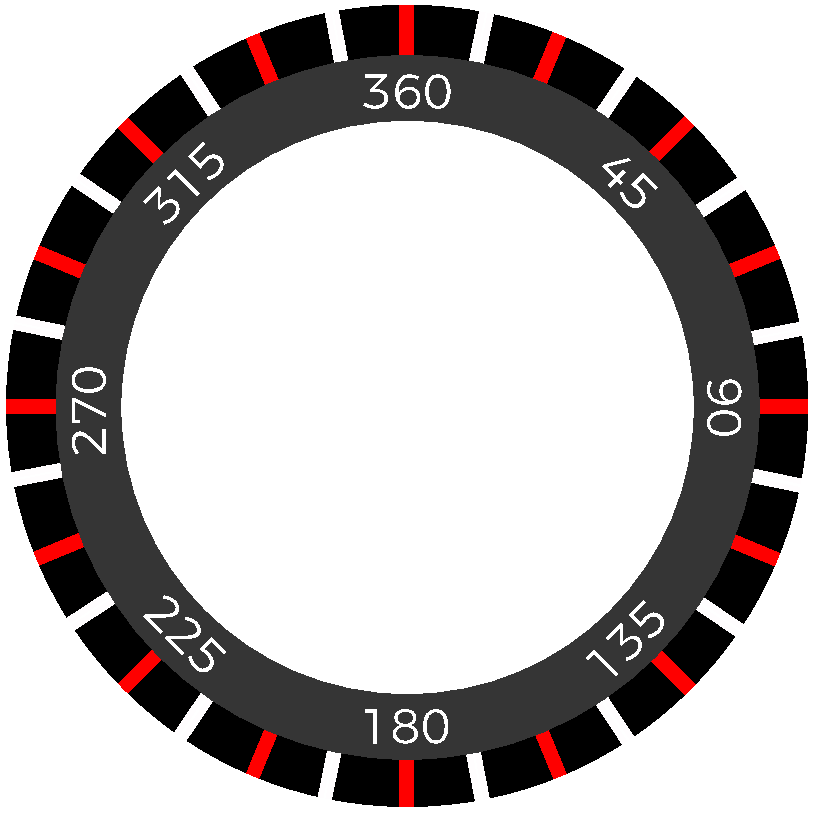
\includegraphics[scale=1.0,angle=0,width=0.37\linewidth]{obrazky-figures/kompas_kostra}
	\caption{Kostra kompasu}
\end{figure}

 

Druhá část kompasu je střelka, která je vložena jako \texttt{<div id="compass\_arrow"\,>} do statické části. Její podoba je demonstrována na obrázku \ref{img:kompas_strelka}. Střelka se  otáčí pomoci transformace kaskádových stylů.

\begin{figure}[h]
	\label{img:kompas_strelka}
	\centering
	
\includegraphics[scale=1.0,angle=0,width=0.4\linewidth]{obrazky-figures/kompas_strelka}
	\caption{Střelka kompasu}
\end{figure}




 


\subsection{Ovládací panel videa}
Ovládací prvky videa jsou vytvářeny pomocí DOM a přidávány do kostry HTML. Celá kostra s atributem \texttt{id=viewer} obsahuje i plátno \texttt{<canvas>}, které se ovládacími prvky překrývá. Při změně velikosti plátna musíme pozice prvků vždy přepočítat. Veškeré operace nad ovládacími prvky zastřešuje funkce \texttt{\createVideoControlls}, kde probíhá i přepočet pozice ovládacích prvků. Jedním ze vstupních argumentů funkce je objekt videa, který je již před-načten do objektové proměnné \texttt{SETTINGS.input.video}. Důvodem jen ten, že  nad objektem funguje celá řada vyvolávaných událostí. Pomocí funkce \texttt{addEventListener()} zde dochází, podobně jako v inicializační části, k vykonávání všech základních operací s videem na základě událostí. Veškeré typy jsou vyvolány interakcí uživatele. Řízeni časové osy a dotazování se na množství načtených dat videa je generováno automaticky. Tlačítko \texttt{fullscreen}, pro zobrazení videa na celou šířku obrazovky, potřebuje přizpůsobit plátno tak, aby nedošlo k deformaci dat, čehož dosáhneme zavoláním funkce \texttt{gl.viewport()}. Ještě je třeba ale uchovávat informace o původní velikosti plátna \texttt{<canvas>}, abychom se mohli z režimu celé obrazovky vrátit. Tyto data jsou uchovány rovněž v objektové proměnné.

Vedle přímých akcí kontrolovaných uživatelem jsou tu ještě  automatické operace prováděné nad videem. Jedná se o detekcí aktivního okna při přehrávání, kdy si program sám ověřuje pomocí funkce \texttt{addEventListener()}  pracující nad objektem \texttt{window}, zda aktuální okno prohlížeče je aktivní. Vše zprostředkovávají události   \texttt{focus} a \texttt{blur}. Událost  \texttt{blur} se spustí ve chvíli, kdy uživatel nemá zobrazené okno s panoramatickým prohlížečem. Tato událost bude mít vliv na video jen v případě, kdy se bude video přehrávat a v takové situaci je i pozastaví, dokud se okno opět nezaktivní událostí \texttt{focus}.

%=========================================================================
\newpage

\subsection{Zorný úhel}
Zorný úhel implementuje funkce \texttt{\createFieldVision}. Výpočet pozice včetně její změny pobíhá stejným způsobem jako u kompasu. HTML element div je v kostře umístěn pod \texttt{id} s názvem  \texttt{field\_vision}. Velikost zorného úhlu je propojena s kolečkem myši tak, že změny zorného úhlu závisí především na přiblíženi, popř. oddálení scény v proměnné \texttt{MOUSE.wheel.delta}. 

Jakmile je do funkce předán argument s velikostí zorného úhlu, tak se pomocí DOM nastaví spolu s  pomocnými vlastnostmi boxu \texttt{field\_vision}, také atribut \texttt{d} v elementu \texttt{<path>}. Celou cestu potřebnou k vykreslení cesty vrací funkce \texttt{fieldVisionCoord()}. Výpočet převodu z polární  do kartézské soustavy souřadnic  se stará operace \texttt{polarToCartesian()}.

Interakce s kolečkem musíme zrealizovat tak, aby při přiblížení scény byl nárůst zorného úhlu rovnoměrný. Konkrétního efektu lze docílit tak, že si zvolíme startovní a cílový úhel, kdy interval mezi nimi je již naše zorné pole. Funkce \texttt{fieldVisionCoord()} proto volá operaci \texttt{polarToCartesian()} hned dvakrát, protože na základě zorného úhlu potřebuje znát oba body v kartézské soustavě souřadnic jak pro začátek, tak konec rozsahu. Jakmile máme oba body spočteny, je možné již sestavit výslednou cestu \texttt{<path>} pro element \texttt{<svg>}. Cesta se bude skládat ze dvou vektorových argumentů pro kreslení křivek. Argument \texttt{M} bude obsahovat hodnotu \texttt{startPoint.x} a \texttt{startPoint.y}, která definuje začátek zorného úhlu. Následuje křivka pomocí argumentu \texttt{A} s příznaky a  koncovým bodem \texttt{(endPoint.x, endPoint.y)}. Definovaná cesta je poté vrácena do funkce \texttt{\createFieldVision} jako prosté pole.




\chapter{Testování}
\label{chapter:5}
Výsledný program bylo třeba otestovat z  hlediska kompatibilita webových prohlížečů  s WebGL nebo s HTML5, až po rozdílnou interpretaci některých vstupních událostí pro periferie počítače. 

Pro testování byl využit jednoduchý nástroj frameworku \texttt{three.js}, který reflektuje aktuální rychlost překreslování scény grafickou kartou. Jedná se konkrétně o třídu \texttt{Stats()}, kterou volá funkce \texttt{DebugThreeStat()} uvedené v knihovně pro externí zdrojové kódy. Vedle měření snímkové frekvence dále disponuje měřením v milisekundách, kolik je zapotřebí času k vykreslení jednoho snímku. Dále velikost alokované paměti v řádech megabajtů.

\section*{Vývojové rostředí a test výkonu}

Program byl vyvíjen na platformě operačního systému Windows 8 s procesorem Intel Core i7 2.4 GHz a GPU Nvidia GT 630m 2GB. Rozlišení LCD displeje $1920 \cdot 1080$px. 

Hlavním prohlížečem pro vývoj sloužil Google Chrome. V přůběhu vývoje byl program také testován v prohlížečích Opera a Firefox. Ověření pak v konečné fázi vývoje programu ještě testováno na operačnímu systému Ubuntu.

Vstupní data, s kterými probíhaly veškeré testy, byly pořízeny sférickou kamerou Ricoh Theta S.

Průměrné naměřené hodnoty při přehrávání dvou minutového videa v režimu celé obrazovky\footnote{V režimu rybího oka.} v různých prohlížečích: 

\begin{center}
	\begin{tabular}{ l | c| c| c  } 
		& \textbf{Firefox} & \textbf{Opera}  & \textbf{Chrome}   \\ 
 		\hline
		Frekvence snímků videa & 28,5 fps & 13,1 fps & 40,3 fps    \\ 
		\hline
		Doba načtení jednoho snímku  & 35 ms & 76 ms & 24 ms  \\ 
		\hline
		Využití paměti & 12  MB & 10  MB & 12  MB   \\ 
		
	\end{tabular}
\end{center}

Testování vykreslování panoramat o rozlišení $1920 \cdot 1080$px v režimu celé obrazovky po dobu jedné minuty:

\begin{center}
	\begin{tabular}{ l | c| c| c  } 
		& \textbf{Firefox} & \textbf{Opera}  & \textbf{Chrome}   \\ 
		\hline
		Frekvence snímků obrázku & 41,2 fps & 41.5 fps & 44 fps    \\ 
		\hline
		Doba načtení jednoho snímku  & 24,2 ms & 24,09 ms & 22,72 ms  \\ 
		\hline
		Využití paměti & 10  MB & 10  MB & 10  MB   \\ 
		
	\end{tabular}
\end{center}

%=========================================================================
\newpage

Stejný test pro panorama a video, ale po vypnutí režimu celé obrazovky\footnote{Zmenšené plátno mělo při testování velikost $1100 \cdot 700$px.}:

\begin{center}
	\begin{tabular}{ l | c| c| c  } 
		& \textbf{Firefox} & \textbf{Opera}  & \textbf{Chrome}   \\ 
		\hline
		Frekvence snímků videa & 49,6 fps & 17,3 fps & 59,9 fps    \\ 
		\hline
		Frekvence snímků obrázku & 59,1 fps & 58,5 fps & 59,6 fps    \\ 
		
	\end{tabular}
\end{center}

\section*{Uživatelské testování}
Testování probíhalo na lidech různých věkových skupin. Uživatelům byl program spuštěn a bylo testováno především jejich chování a interakce s panoramatickým prohlížečem. Důraz byl kladen na rychlost seznámení se s uživatelským rozhraním a způsobem jeho ovládání.

Mezi základní úkony patřilo ovládání pozorovatele ve scéně pomocí myši, dále změna zdroj dat, který se právě zpracovával. Ovládání doplňovala ještě klávesnice, přičemž  u videa navíc přibyla i časová osa včetně kontextových tlačítek. 


\section*{Shrnutí testování}
Jak již lze pozorovat, ve všech testech Opera velice ztrácí, zejména v přehrávání videa, kdy video nebylo při přehrávaní vůbec plynulé, a to ani po vypnutí režimu celé obrazovky. Naproti tomu prohlížení sférického videa v prohlížeči Firefox bylo znatelně plynulejší a ve všech módech prohlížení si vedl obstojně. Nejlépe ale vše fungovalo v prohlížeči Chrome, kde bylo přehrávání a prohlížení ve všech módech vždy plynulé. 

Z hlediska uživatelského testování vyšlo najevo, že se uživatelé nejrychleji z grafických prvků seznámili se zorným úhlem, kdy interakce pomocí myši korelovala odpovídajícím způsobem se scénou. Ovládání pomocí myši nejevilo zjevné problémy hlavně u mladších uživatelů. Celkově program působil na respondenty příjemným dojmem a některé jejich návrhy, popř. připomínky budou sloužit jako námět v budoucím vývoji.
 
\chapter{Závěr}
\label{chapter:6}

\section{zhodnocení  dosažených výsledků s  vyznačeným vlastním přínosem studenta}
Účelem práce bylo implementovat prohlížeč ve WebGL, který je schopen přehrát sférická videa v různých režimech. Hlavně tedy v režimu, který by v jiných prohlížečích byl velice zkreslen, protože by nepodporoval režim rybího oka. Implementovaný prohlížeč je schopen tento režim zvládnout bez pomocí externích programů, popř. konvertorů, které dává k dispozici přímo výrobce 360 stupňové kamery. Díky programu tedy již externí konvertor není potřeba a výstup z kamery lze prohlížet okamžitě po natočení.


\section{náměty(zdroje inspirace) vycházející ze zkušeností s řešeným projektem}
\section{návaznosti na právě dokončené projekty}


\section{zhodnocení z pohledu dalšího vývoje projektu}
Vylepšení programu by mohlo přijít spolu s novou verzí WebGL, která v době implementace této práce ještě nebyla oficiálně vydána. Nová verze disponuje širší škálou možností a otevírá nové možnosti, jak program vylepšit a optimalizovat. Projekt jako takový má velký potenciál, jak již bylo uvedeno v úvodu práce, v současné době je trendem  rozšiřování možnosti prohlížení. Dalším vylepšením by mohla být přidána širší podpora zařízení, jako např. ty, které disponují více kamerami, aby pokryly lépe celou sféru, zde by byla velice zajímaví implementace, kdy  by si musela poradit s více záběry a mapovat je na jeden sférický model. Popřípadě přidat automatické rozeznávání objektu na kameře, apod.

Z hlediska dalšího vývoje je velice výhodná implementace bez přítomností frameworků, které práci s WebGL zastřešují. Důvod je zřejmý, není třeba v takové problematice používat všechny funkce, čímž se velikost programu jako takového zmenší a kód bude přehlednější.
 


%=========================================================================
